
\section{Background estimation}
\label{sec:bkgd}
\subsection{Irreducible background}
\label{sec:irrbkgd}
\subsubsection{\qqZZ~ Modelling}

The \qqZZ~ background is generated at NLO, while the fully differential cross section has been computed at 
NNLO~\cite{Grazzini2015407}, but is not yet available in a partonic level event generator. Therefore NNLO/NLO 
$k$-factors for the \qqZZ~background process are applied to the {\sc powheg} sample. The inclusive cross 
sections obtained using the same PDF and renormalization and factorization scales as the {\sc powheg} sample
at LO, NLO, and NNLO are shown in Table~\ref{tab:qqZZXS}. The NNLO/NLO $k$-factors are applied in the analysis
differentially as a function of $m(\cPZ\cPZ)$ to both signal and \qqZZ~background samples. Also, additional NLO/LO~$k$-factors 
are applied to the {\sc MadGraph5} signal samples and can be seen in
Figure~\ref{fig:qqZZKfactor}.

\begin{table}[h]
    \centering
    \begin{tabular}{|l|c|c|} 
\hline %----------------------------------------------------------------
QCD Order  & $\sigma_{2\ell2\ell^{\prime}} (\mathrm{fb})$  & $\sigma_{4\ell} (\mathrm{fb})$  \\
\hline %----------------------------------------------------------------
LO    & 218.5$^{+16\%}_{-15\%}$ & 98.4$^{+13\%}_{-13\%}$ \\
NLO   & 290.7$^{+5\%}_{-8\%}$   & 129.5$^{+4\%}_{-6\%}$ \\
NNLO  & 324.0$^{+2\%}_{-3\%}$   & 141.2$^{+2\%}_{-2\%}$ \\
\hline %----------------------------------------------------------------
    \end{tabular}
    \caption{Cross sections for \qqZZ~ production at 13 \TeV}
    \label{tab:qqZZXS}
\end{table}

%=======
\begin{figure}[!htb]
\vspace*{0.3cm}
\begin{center}
\includegraphics[width=0.68\textwidth]{Figures/IrrBkg/Kfactor_qqZZ_mZZ.pdf}
%\includegraphics[width=0.48\textwidth]{Figures/IrrBkg/K_ewk_qqZZ.pdf} 
\caption{NNLO/NLO(Black)and NLO/LO(Red) QCD $k$-factor for the \qqZZ~ background as a function of $m(ZZ)$ for the $4\mu$ final states. 
%Right: NLO/NLO electroweak $k$-factor for the \qqZZ~ background as a function of $m(ZZ)$.
\label{fig:qqZZKfactor}}
\end{center}
\end{figure}


\subsubsection{\ggZZ~ Modelling}

Event simulation for the $\ggZZ$ background is done at LO with the generator \MCFM~7.0~\cite{MCFM,Campbell:2011bn,Campbell:2013una}.
Although no exact calculation exists beyond the LO for the $\ggZZ$ background, 
it has been recently shown~\cite{Bonvini:1304.3053} 
that the soft collinear approximation is able to describe the background cross section and the 
interference term at NNLO\@. Further calculations also show that the K factors are very similar at NLO, 
NNLO and interference terms~\cite{Li:2015jva} for the SM Higgs production by gluon fusion (\ggH) and 
$\ggZZ$ background~\cite{Melnikov:2015laa}. Therefore, the K factor is used for $\ggZZ$ background as of
Higgs production(\ggH)~\cite{Passarino:1312.2397v1}. The NNLO K factor for~\ggH~is obtained as a function 
of \mass{4\ell}  using the \textsc{hnnlo}~v2 Monte Carlo 
program~\cite{Catani:2007vq,Grazzini:2008tf,Grazzini:2013mca} by calculating the NNLO and LO 
$\Pg\Pg\to\PH\to2\ell2\ell^\prime$ cross sections at the small $\PH$ boson decay width of $4.07$~\MeV 
and taking their ratios. The NNLO K factors, as 
well as the NLO K factors and the cross sections from which they are derived, are illustrated in Fig.~\ref{fig:ggHZZXsecKfactor}, 
along with the NNLO, NLO and LO cross sections at the SM $\PH$ boson decay width~\cite{Heinemeyer:2013tqa}.
 
\begin{figure}[!htb]
\centering
\includegraphics[width=0.48\linewidth]{Figures/IrrBkg/cCompare_hnnlo_ggHZZ2l2l_xsec.pdf}
\includegraphics[width=0.48\linewidth]{Figures/IrrBkg/cCompare_hnnlo_ggHZZ2l2l_narrowwidth_xsec.pdf}\\
\includegraphics[width=0.48\linewidth]{Figures/IrrBkg/cCompare_hnnlo_ggHZZ2l2l_narrowwidth_kfactor.pdf}
\caption{$\Pg\Pg\to\PH\to2\ell2\ell^\prime$ cross sections at NNLO, NLO and LO at each $\PH$ boson pole mass using the SM $\PH$ boson decay width  (top \cmsLeft) or at the fixed and small decay width of $4.07$~MeV (top \cmsRight). The cross sections using the fixed value are used to obtain the K factor for ~$\ggZZ$~ process as a function of $\mllll$ (bottom.)}
\label{fig:ggHZZXsecKfactor}
\end{figure}


\subsection{Reducible background}
\label{sec:redbkgd}

The method (OS method) employed to estimate the reducible background (\zx) is the same as in~\cite{AN-16-442,AN-17-342}, with 
addition validations in data sideband to ensure consistent agreement between data and \zx predictions.
\zx originates from physics processes with one or more mis-identified non-prompt 
leptons, mimicing four-prompt-lepton signatures. Non-isolated electrons and muons from heavy-flavour hadrons, 
mis-identified jets and electrons from $\gamma$ conversion are sources of non-prompt leptons.

In essence, fake rates (\frEl and \frMu), defined as the probability for a fake lepton to pass the tight 
lepton selection given that the fake lepton already passes the loose selection, are measured with data in 
bins of lepton \pt, for electrons and muons separately. These probabilities are then applied in dedicated 
control sample enriched in fake leptons to prediction background contributions in the signal region.

For the region with $\mass{Z2} < 12~\GeV$, $\Delta R$ between two loose leptons could be less than the isolation cone, 
as shown in Figure~\ref{fig:mZ2_DeltaR34_Data16} in the control region enriched in events with two tight and two loose leptons. 
Due to the overlapping of isolation cones, fake rates associated with these two loose leptons could be correlated, 
while the OS method assumes uncorrelated fake rates.
\begin{figure}[!htb]
\begin{center}
    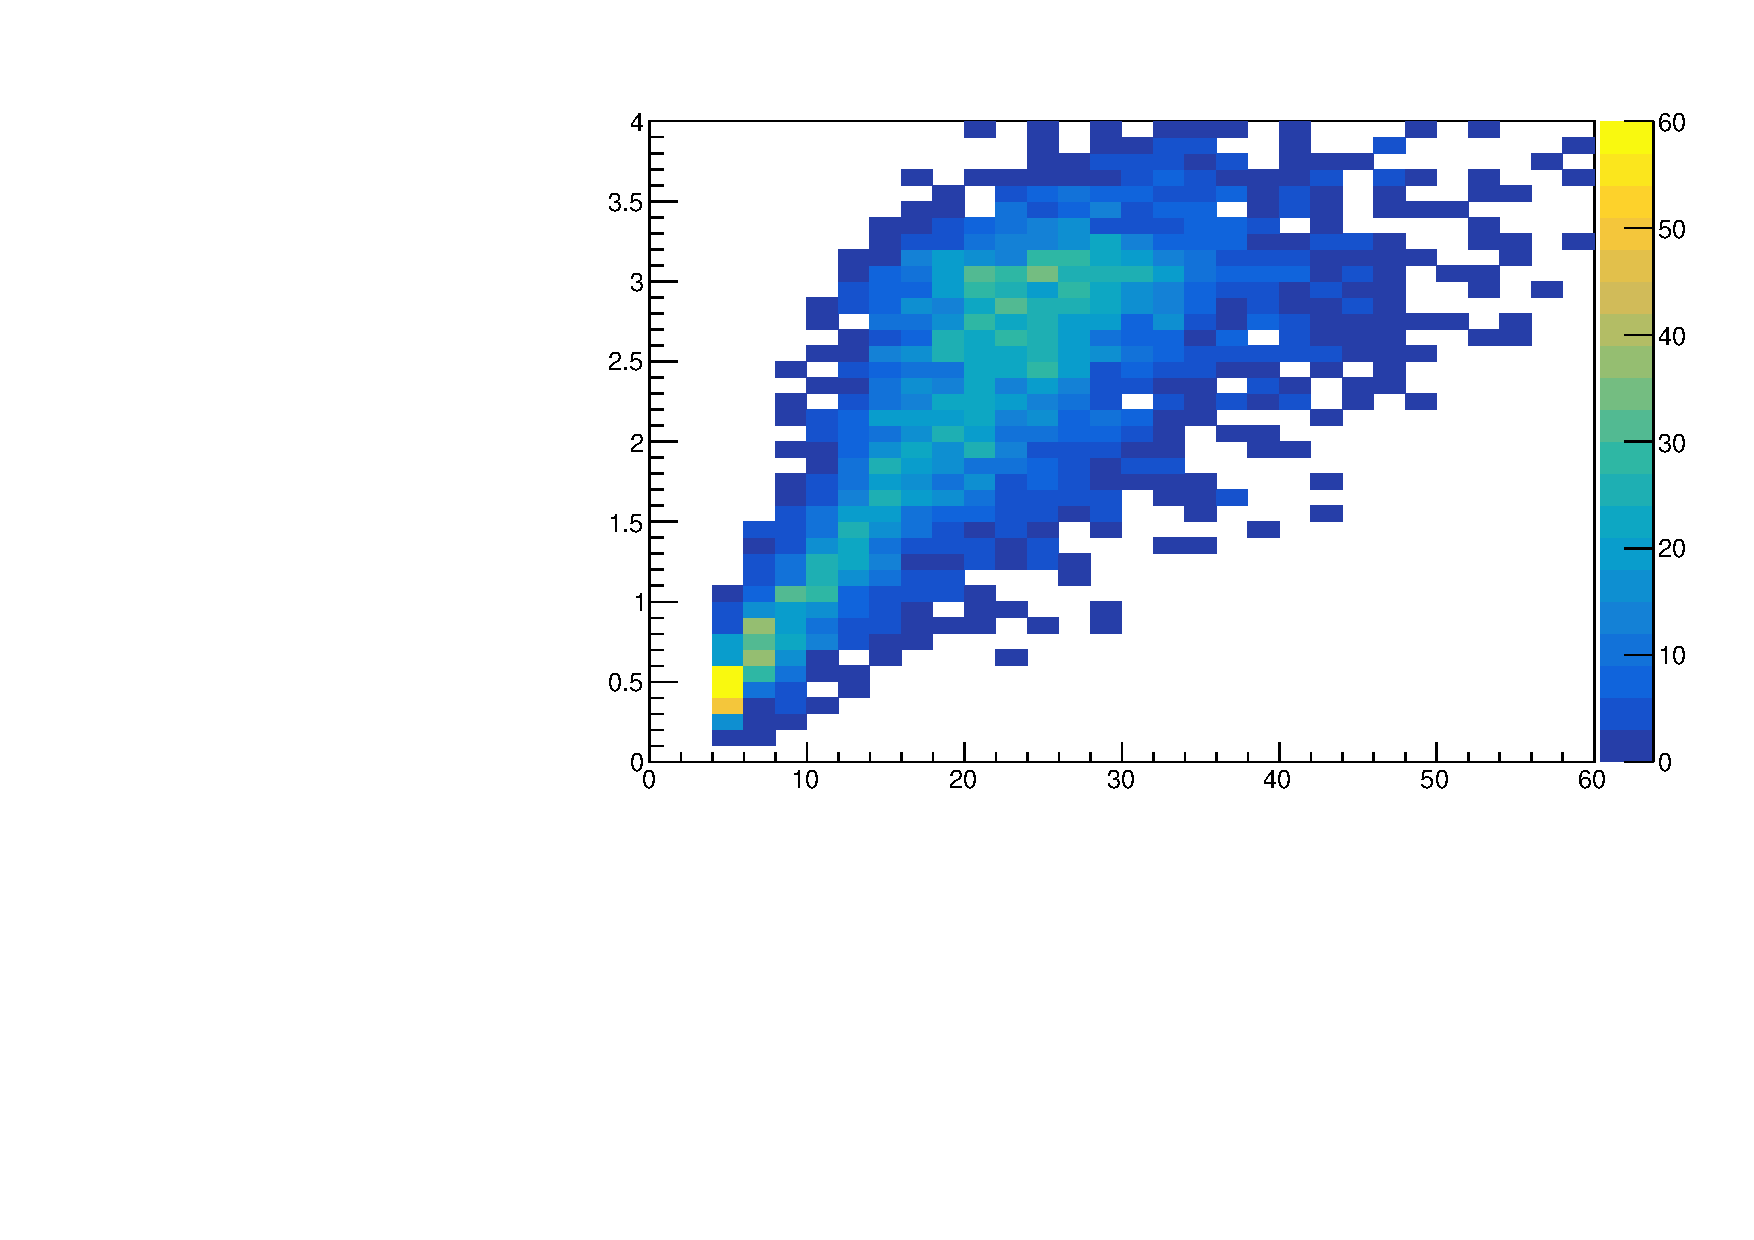
\includegraphics[width=0.80\textwidth]{Figures/RedBkg/Data_Run2016_Z2_mass_vs_DeltaR34_2p2f.pdf}
    \caption{
    \mass{Z2} vs $\Delta R_{\mathrm{loose leptons}}$ the control region enriched in events with two tight and two loose leptons.  
    \label{fig:mZ2_DeltaR34_Data16}
    }
\end{center}
\end{figure}
Therefore, dedicated validations are performed with data in \mass{4\ell} sidebands and the Wrong-Flavour-Charge 
(WrongFC) control region to check closure of the method, especially in the $\mass{Z2} < 12~\GeV$ region, in which 
non-prompt leptons are within the isolation cone and fake rates could be correlated between them. Furthermore, 
a dedicated procedure is also used to estiamte the effect with correlated fake rates and corresponding 
systematic uncertainties are derived.

\subsubsection{Fake rate measurement}

To measure the \frEl and \frMu, a control sample enriched in $Z(\ell\ell)+e$ and $Z(\ell\ell)+\mu$ are selected. This control 
samples are dominated by events with a $Z$ boson and a fake lepton. Events are required to have two same flavour, 
opposite signed leptons with $\pt > 20/10~\GeV$ with tight selection criteria and an lepton satisfying 
loose selection criteria. To reduce low mass resonance, the invariant masses of this loose lepton and each tight lepton 
are required to be $m_{2\ell} > 4~\GeV$. The invariant mass formed by the two tight leptons is also required to be 
$|M(\ell_{1},\ell_{2}) - M_{Z}| < 7~\GeV$ to reduce contributions from photon conversions.

Fake rates are measured in bins of lepton \pt, and separately in the barrel and endcap region, as shown in Figure~\ref{fig:os_fakerates_16}-\ref{fig:os_fakerates_18}.
\begin{figure}[!htb]
\begin{center}
    \subfigure [] {\includegraphics [width=0.45\textwidth]{Figures/RedBkg/FakeRate2016/FR_electrons_ptl3_DataallTR.pdf}}
    \subfigure [] {\includegraphics [width=0.45\textwidth]{Figures/RedBkg/FakeRate2016/FR_muons_ptl3_DataallTR.pdf}}
  \caption{
Fake rates as a function of the probe \pt for  electrons (a) and muons (b) which satisfy the loose selection criteria, measured in
a $Z(\ell\ell)+\ell$ sample with data in Run 2016.
The barrel selection includes electrons (muons) up to $|\eta|$ = 1.479 (1.2).
}
\label{fig:os_fakerates_16}
\end{center}
\end{figure}

\begin{figure}[!htb]
\begin{center}
    \subfigure [] {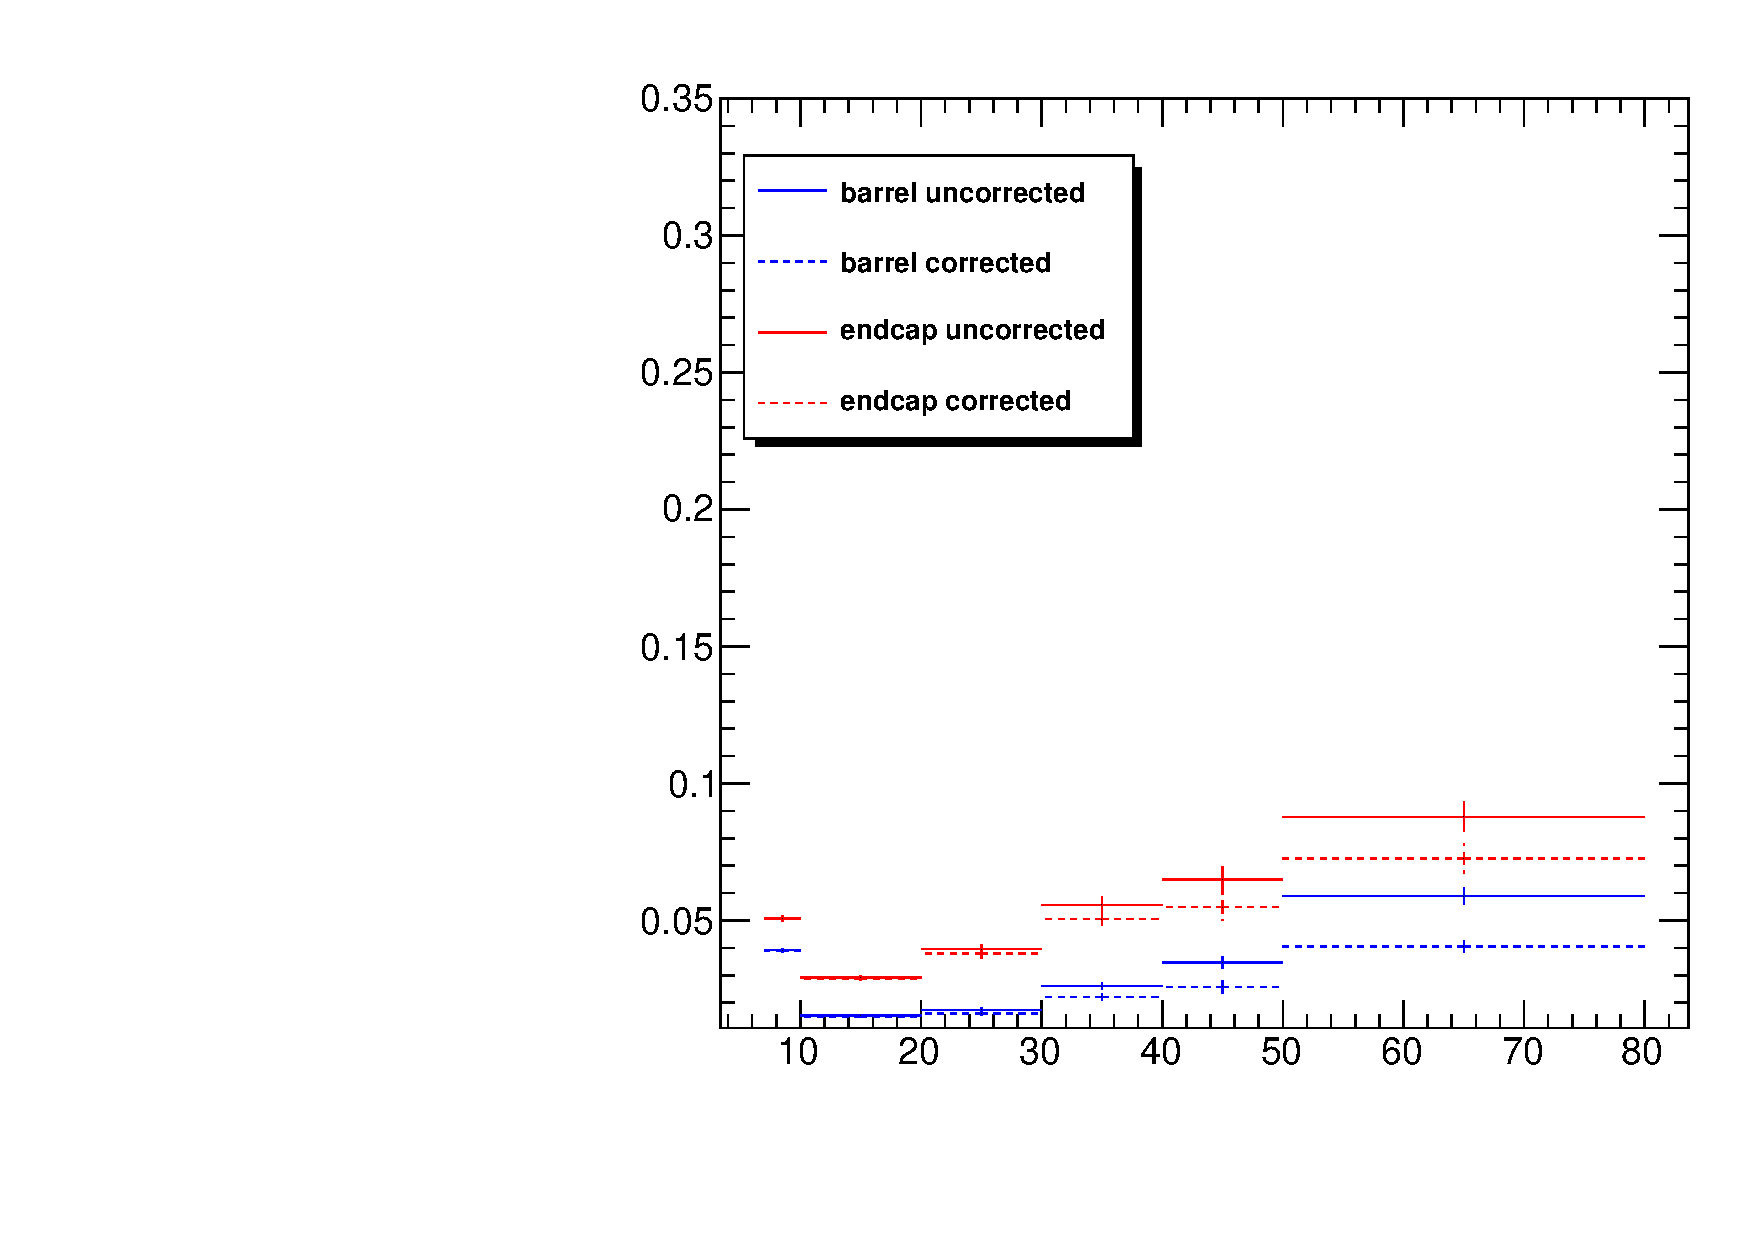
\includegraphics [width=0.45\textwidth]{Figures/RedBkg/FakeRate2017/FR_OS_electrons_2may18.pdf}}
    \subfigure [] {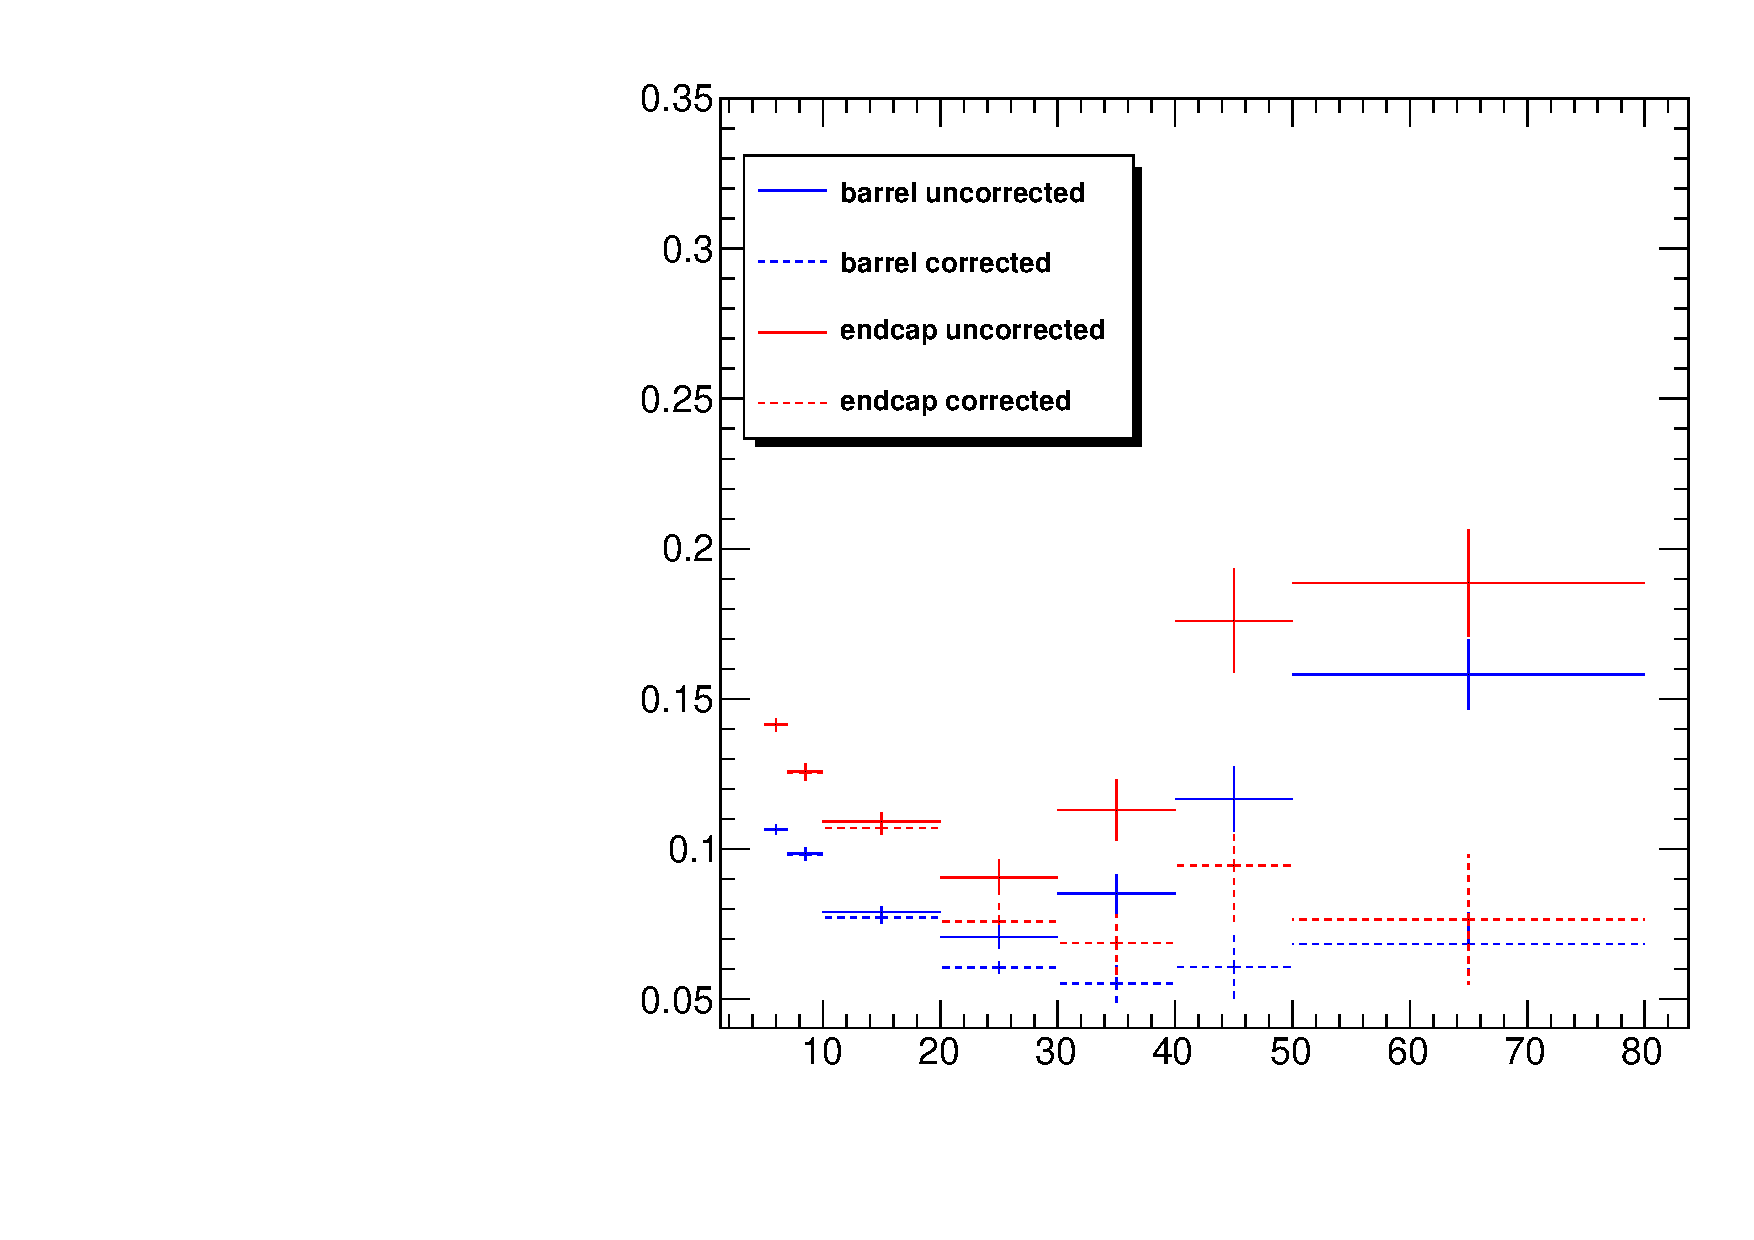
\includegraphics [width=0.45\textwidth]{Figures/RedBkg/FakeRate2017/FR_OS_muons_2may18.pdf}}

    \caption{
        Fake rates as a function of the probe \pt for  electrons (a) and muons (b) which satisfy the loose selection criteria, measured in
        a $Z(\ell\ell)+\ell$ sample with data in Run 2017.
        The barrel selection includes electrons (muons) up to $|\eta|$ = 1.479 (1.2).
    }
\label{fig:os_fakerates_17}
\end{center}
\end{figure}

\begin{figure}[!htb]
\begin{center}
    \subfigure [] {\includegraphics [width=0.45\textwidth]{Figures/RedBkg/FR_electrons_ptl3_DataallTR.pdf}}
    \subfigure [] {\includegraphics [width=0.45\textwidth]{Figures/RedBkg/FR_muons_ptl3_DataallTR.pdf}}
    \caption{
        [Placeholder for 2018] Fake rates as a function of the probe \pt for  electrons (a) and muons (b) which satisfy the loose selection criteria, measured in
        a $Z(\ell\ell)+\ell$ sample with data in Run 2017.
        The barrel selection includes electrons (muons) up to $|\eta|$ = 1.479 (1.2).
    }
\label{fig:os_fakerates_18}
\end{center}
\end{figure}

\subsubsection{Fake rate application}
Two control samples are defined by requiring the same selections as the signal region, but inverting the 
lepton selection criteria. The first control sample is obtained by requiring two leptons forming the Z2 
candidate to pass loose selection criteria but not tight criteria. This control sample, denoted as 2P2F, 
is expected to be dominated by \dy, \ttNew and \zg events. The second control sample, denoted as 3P1F, is 
obtained by one of the four leptons passing only loose criteria instead. The 3P1F is expected to be dominated 
by similar physics processes as in 2P2F but with different relative compositions, and \wz events.
These two control samples enriched in fake leptons are used to estimate the \zx contribution in the signal 
region.

Various distributions of events for the 2P2F and 3P1F control sample are shown in Fig.~\ref{fig:mZ2_2P2F_dataMC_16}-\ref{fig:DeltaR_dataMC_16}. 

\begin{figure}[!htb]
\begin{center}
    {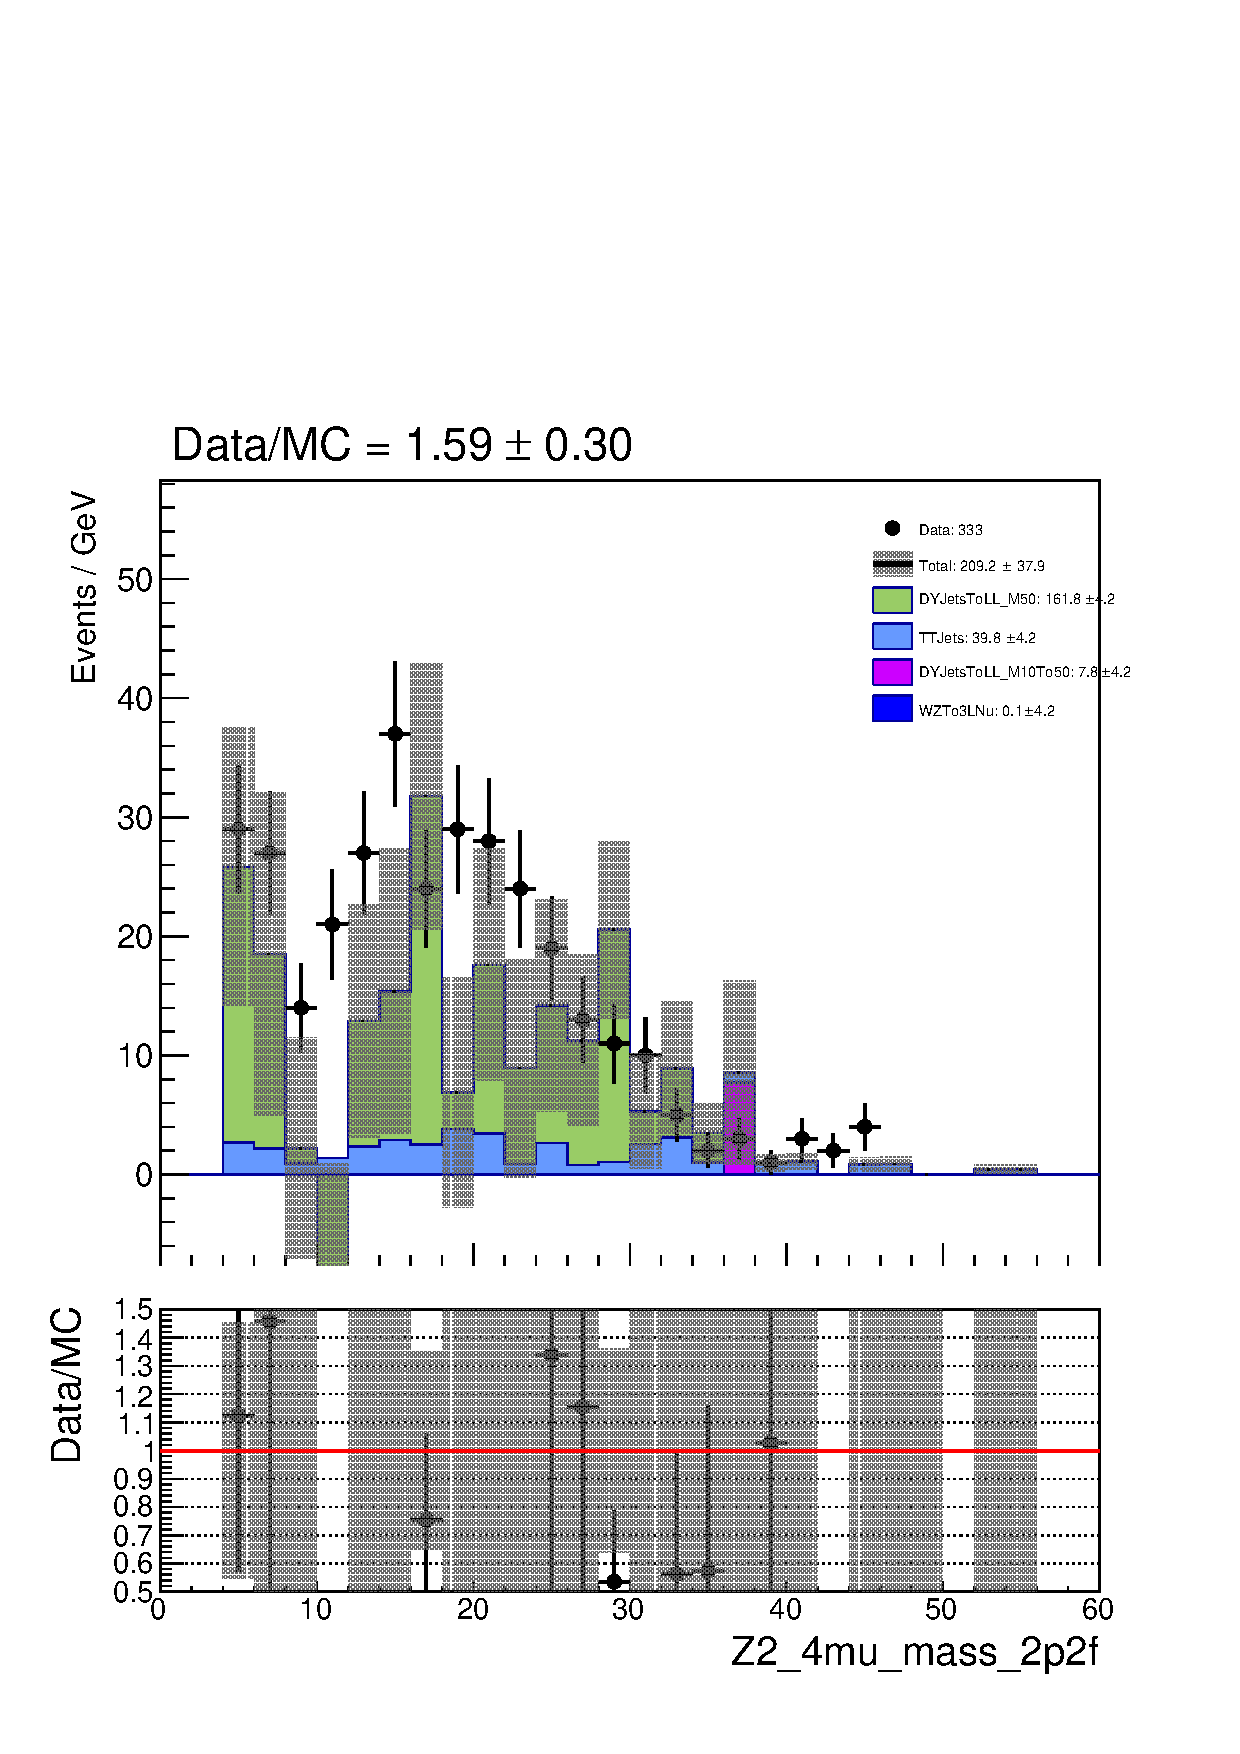
\includegraphics [width=0.45\textwidth] {Figures/RedBkg/2P2F/Z2_4mu_mass_2p2f.pdf}}
    {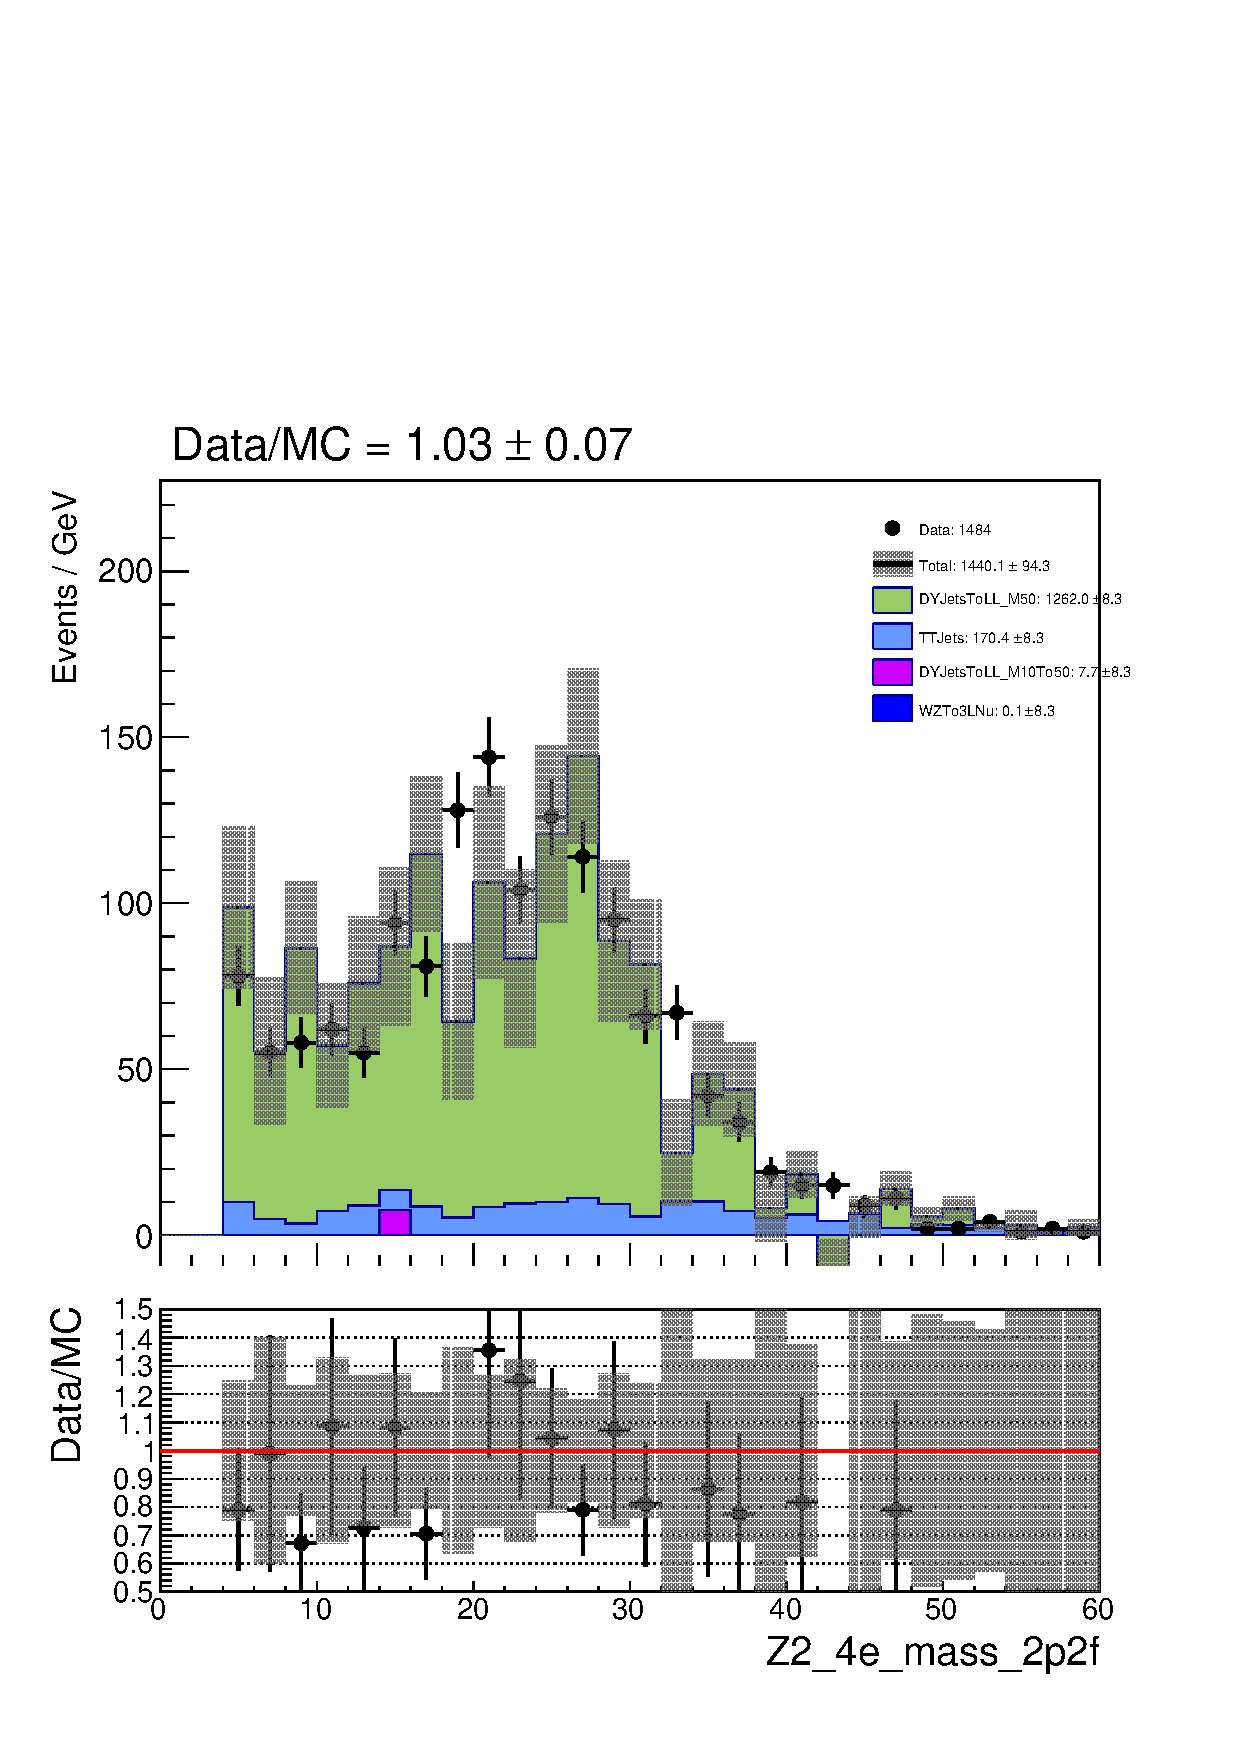
\includegraphics [width=0.45\textwidth] {Figures/RedBkg/2P2F/Z2_4e_mass_2p2f.pdf}} \\
    {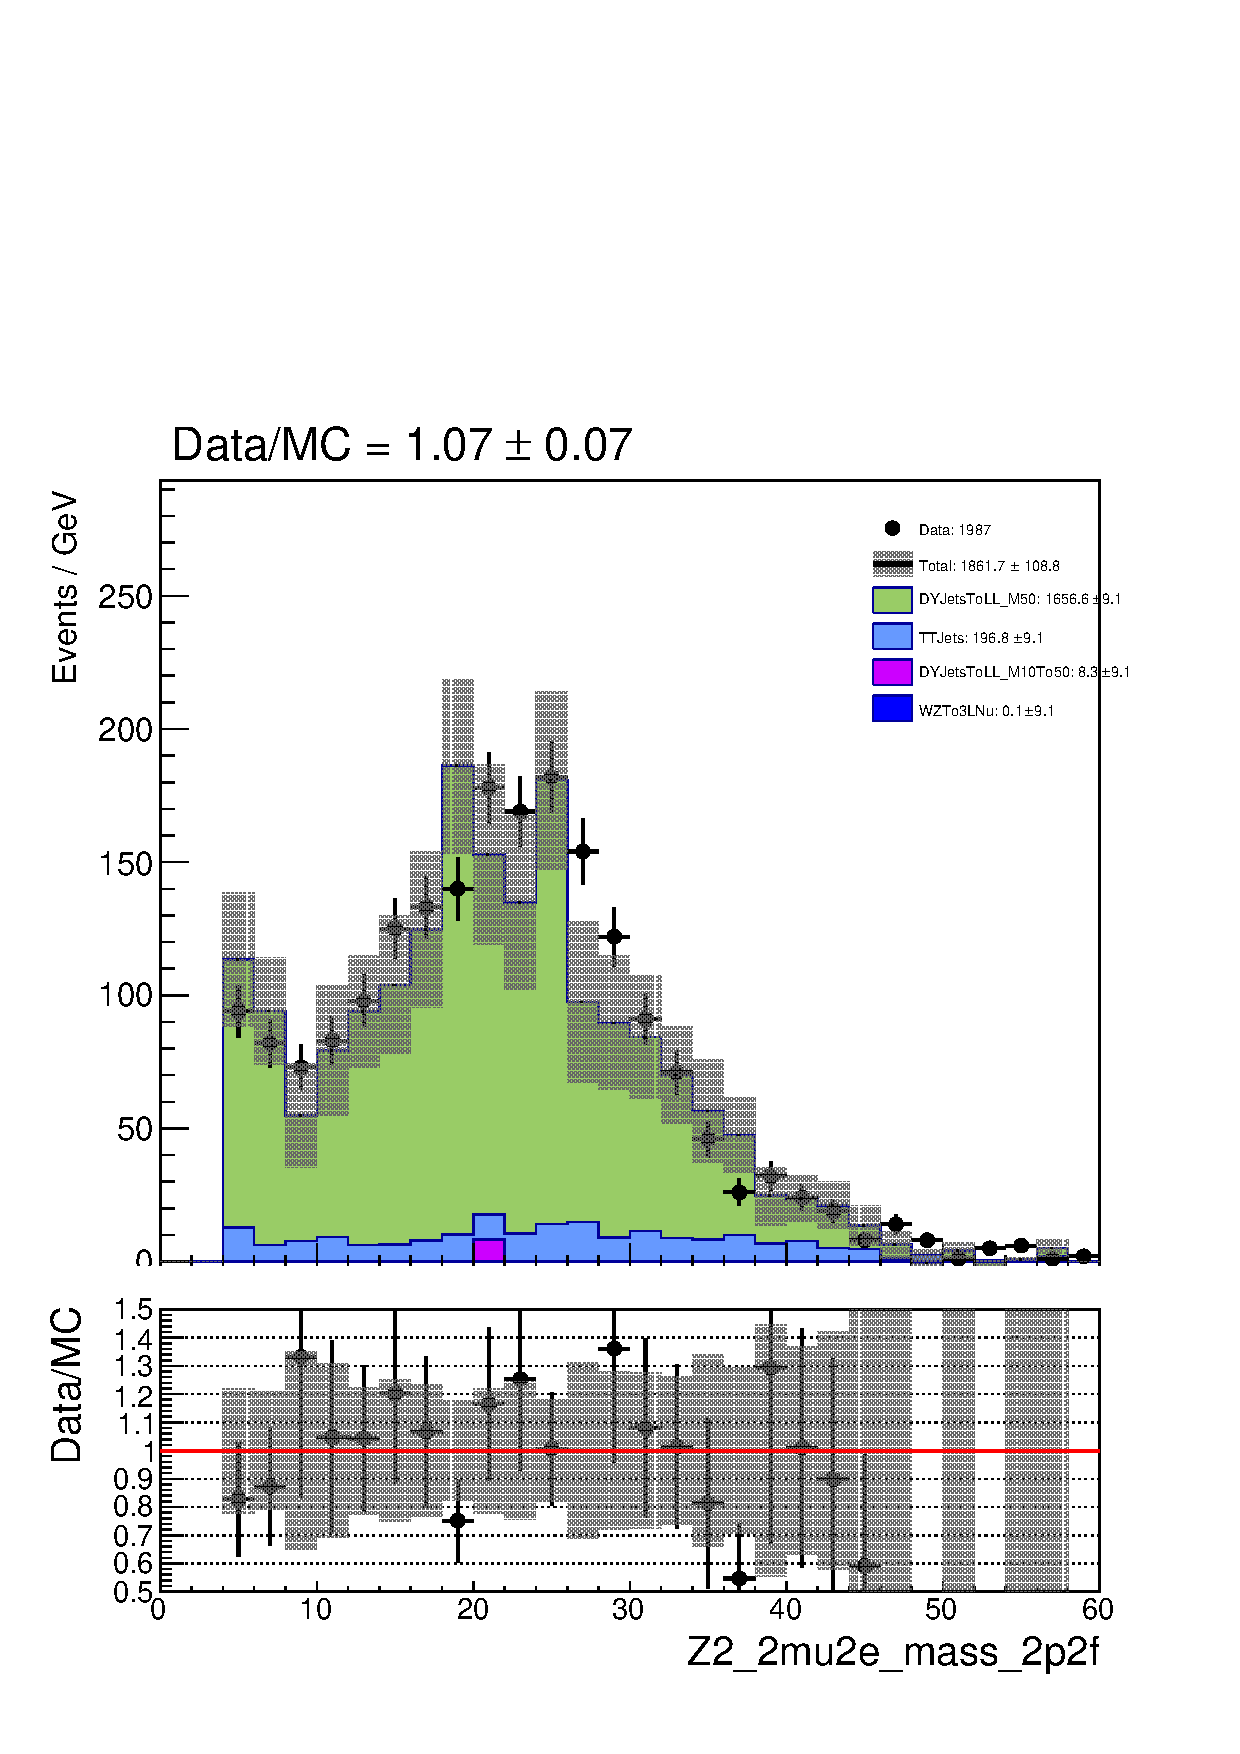
\includegraphics [width=0.45\textwidth] {Figures/RedBkg/2P2F/Z2_2mu2e_mass_2p2f.pdf}}
    {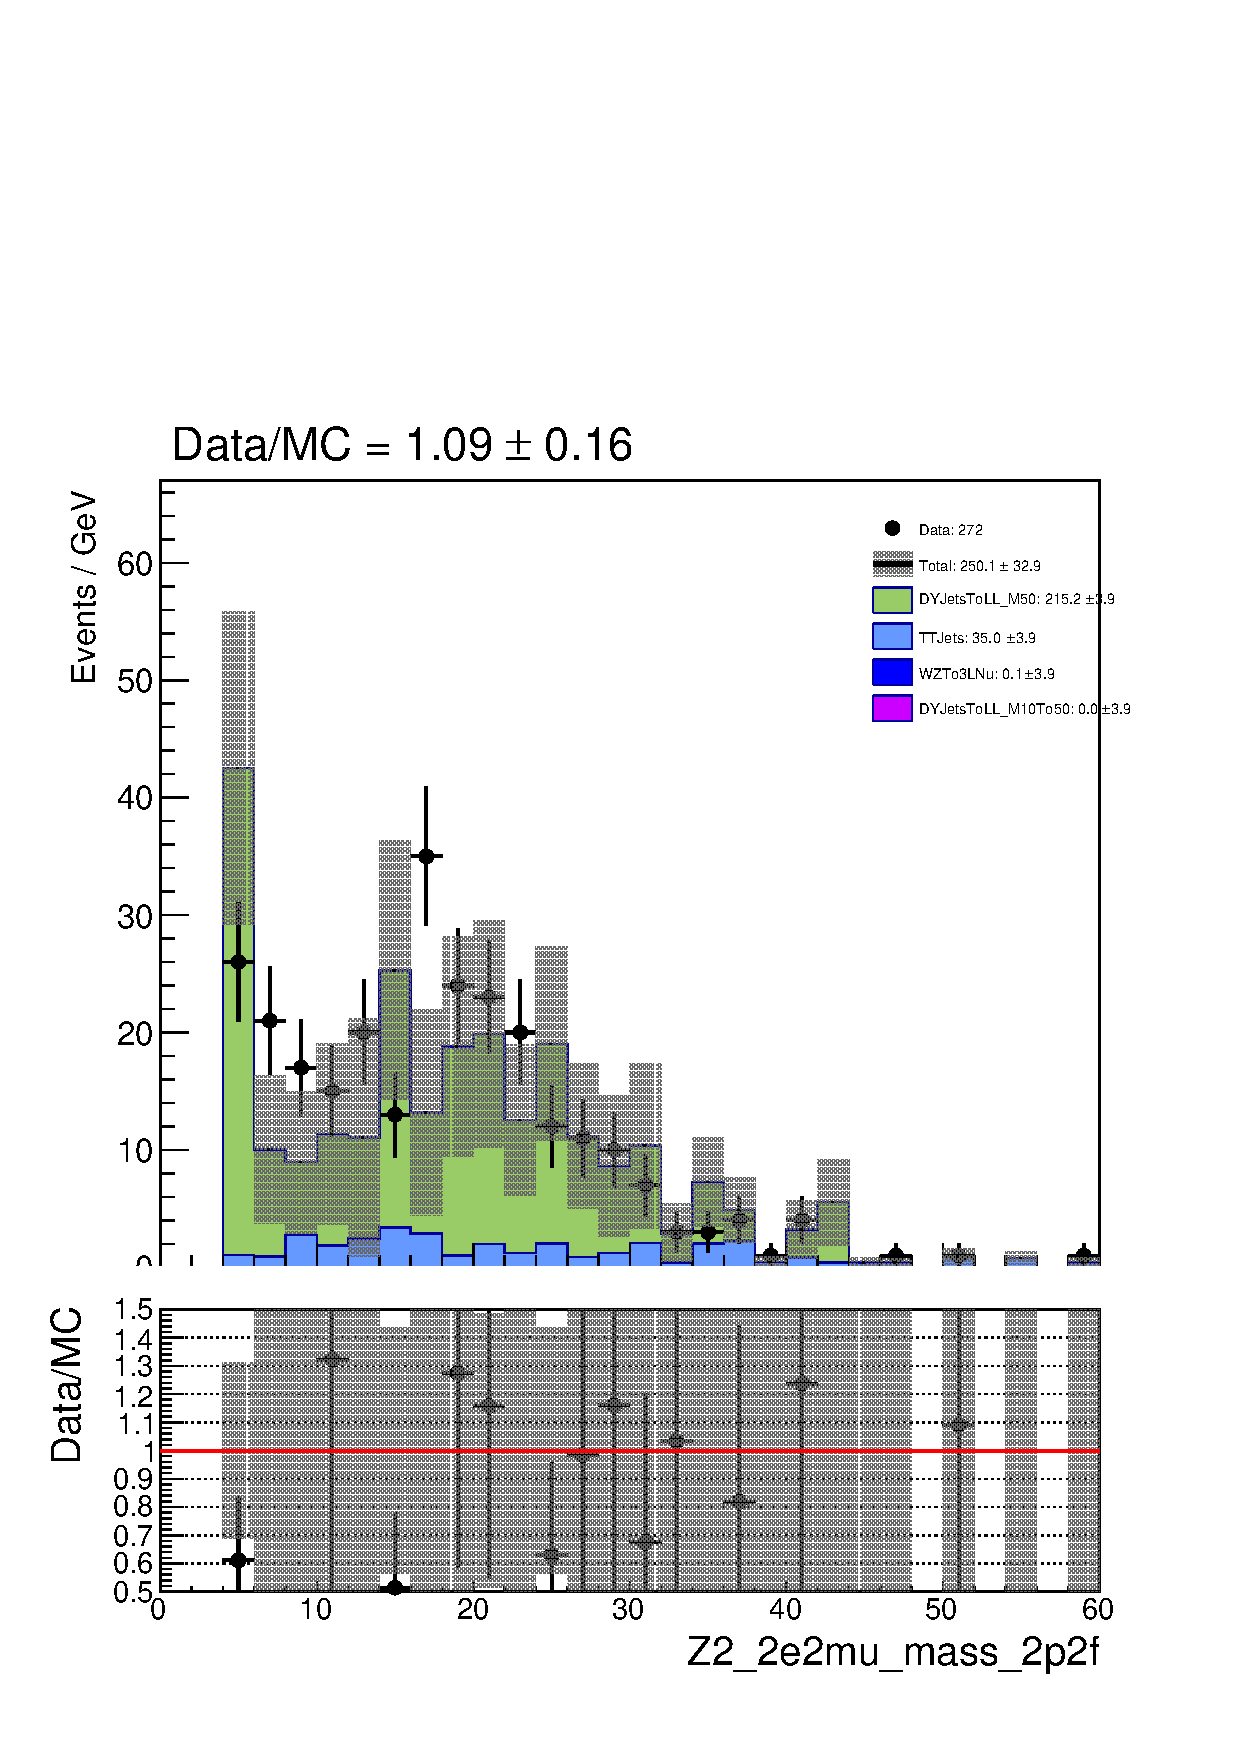
\includegraphics [width=0.45\textwidth] {Figures/RedBkg/2P2F/Z2_2e2mu_mass_2p2f.pdf}} \\
    \caption{
        \mass{Z2} distribution of the events selected in the 2P2F control sample with data in Run 2016, 
        (top left)  $4\mu$ , (top right) $4e$ , (bottom left)  $2\mu2e$ and (bottom right)  $2e2\mu$ channels.
    }
\label{fig:mZ2_2P2F_dataMC_16}
\end{center}
\end{figure}

\begin{figure}[!htb]
\begin{center}
    {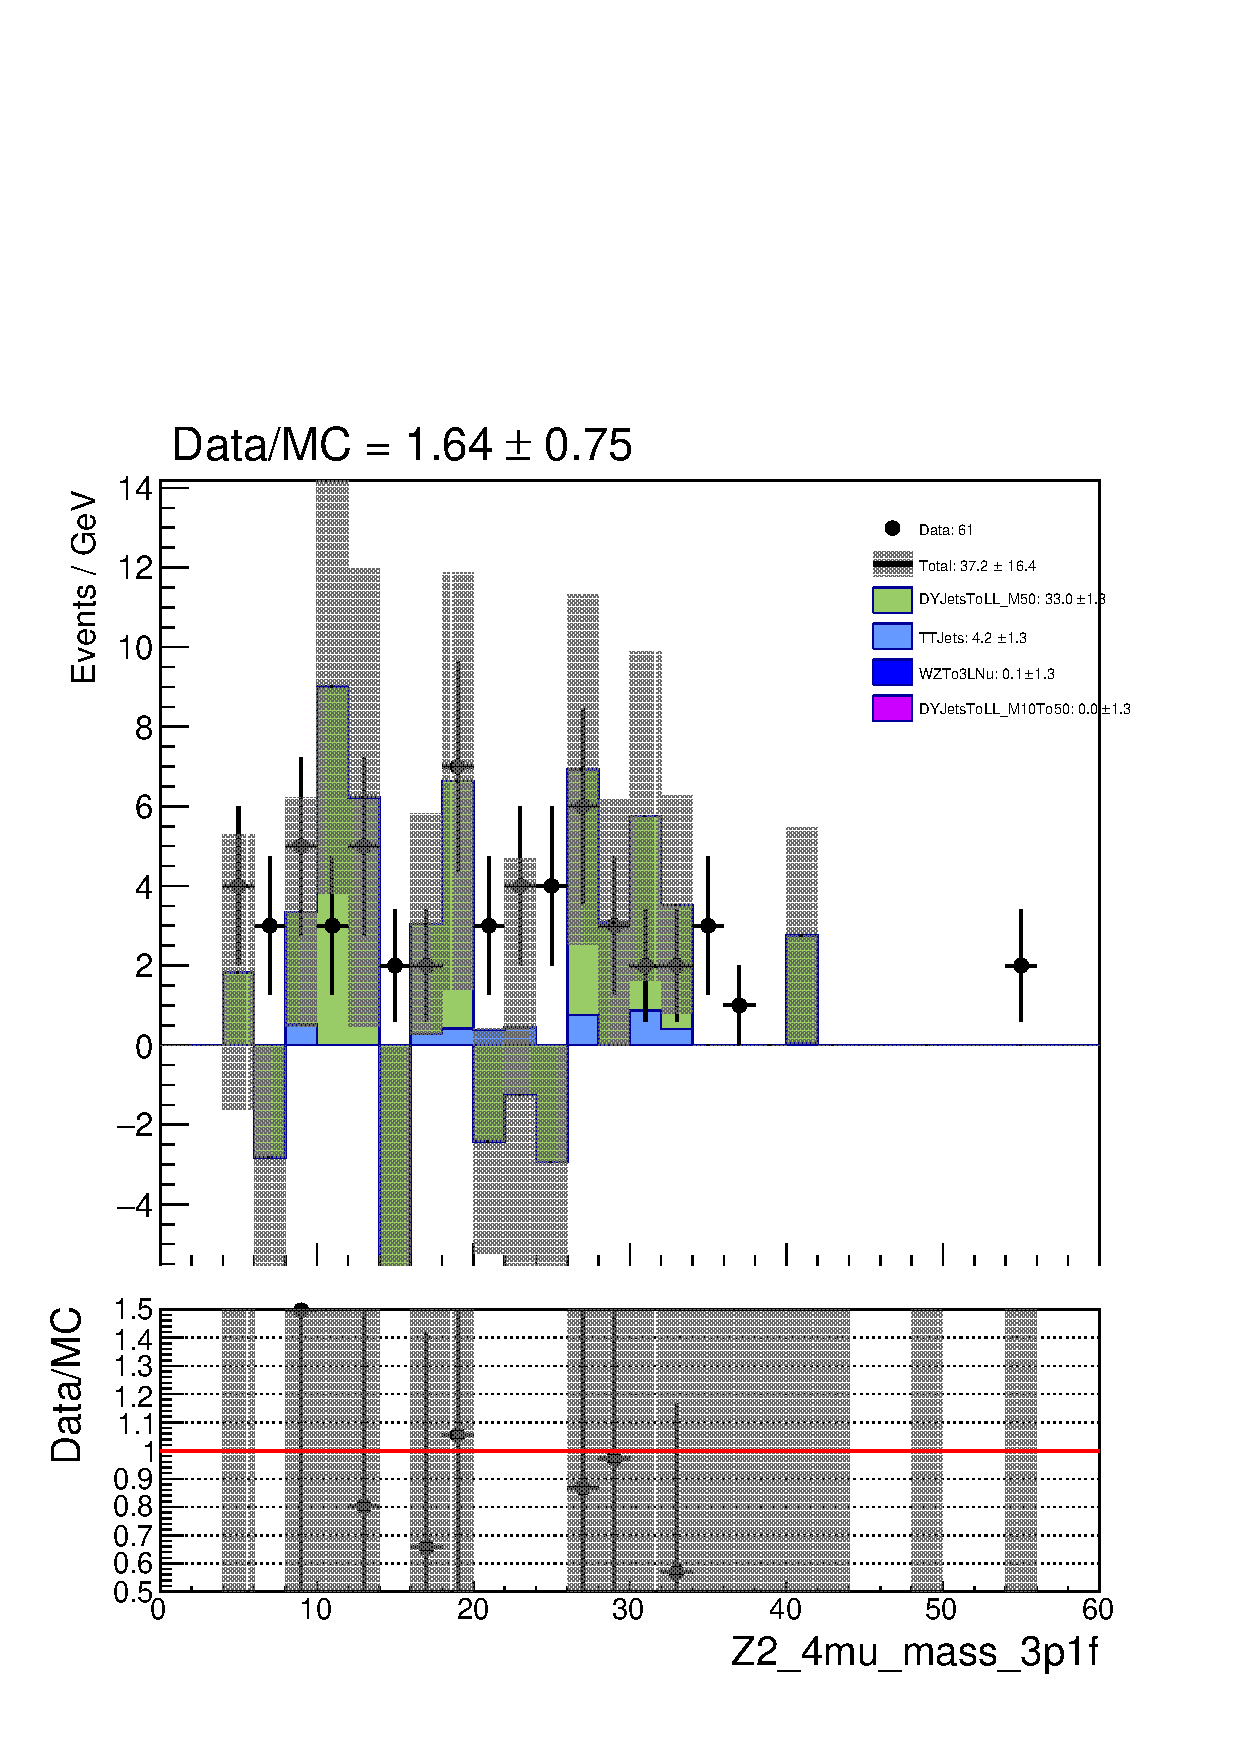
\includegraphics [width=0.45\textwidth] {Figures/RedBkg/3P1F/Z2_4mu_mass_3p1f.pdf}}
    {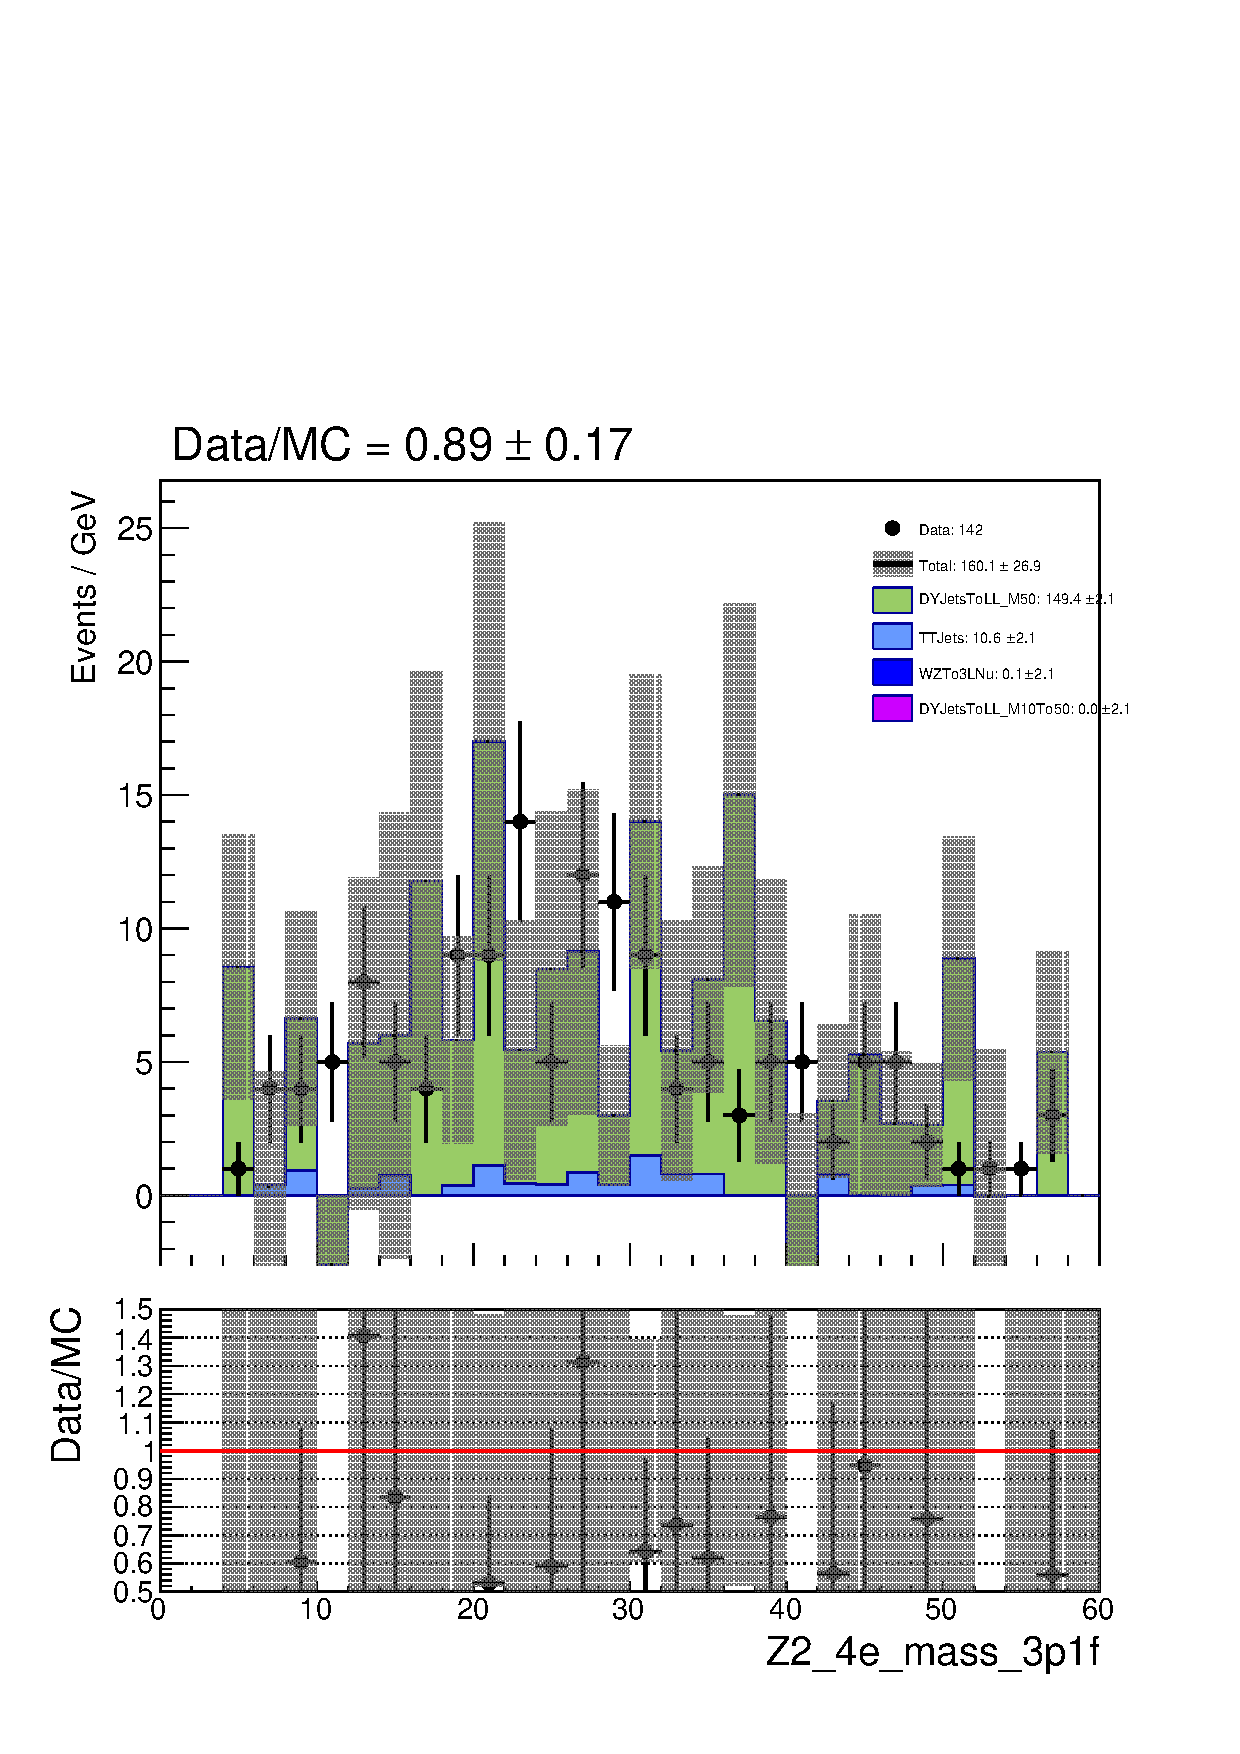
\includegraphics [width=0.45\textwidth] {Figures/RedBkg/3P1F/Z2_4e_mass_3p1f.pdf}} \\
    {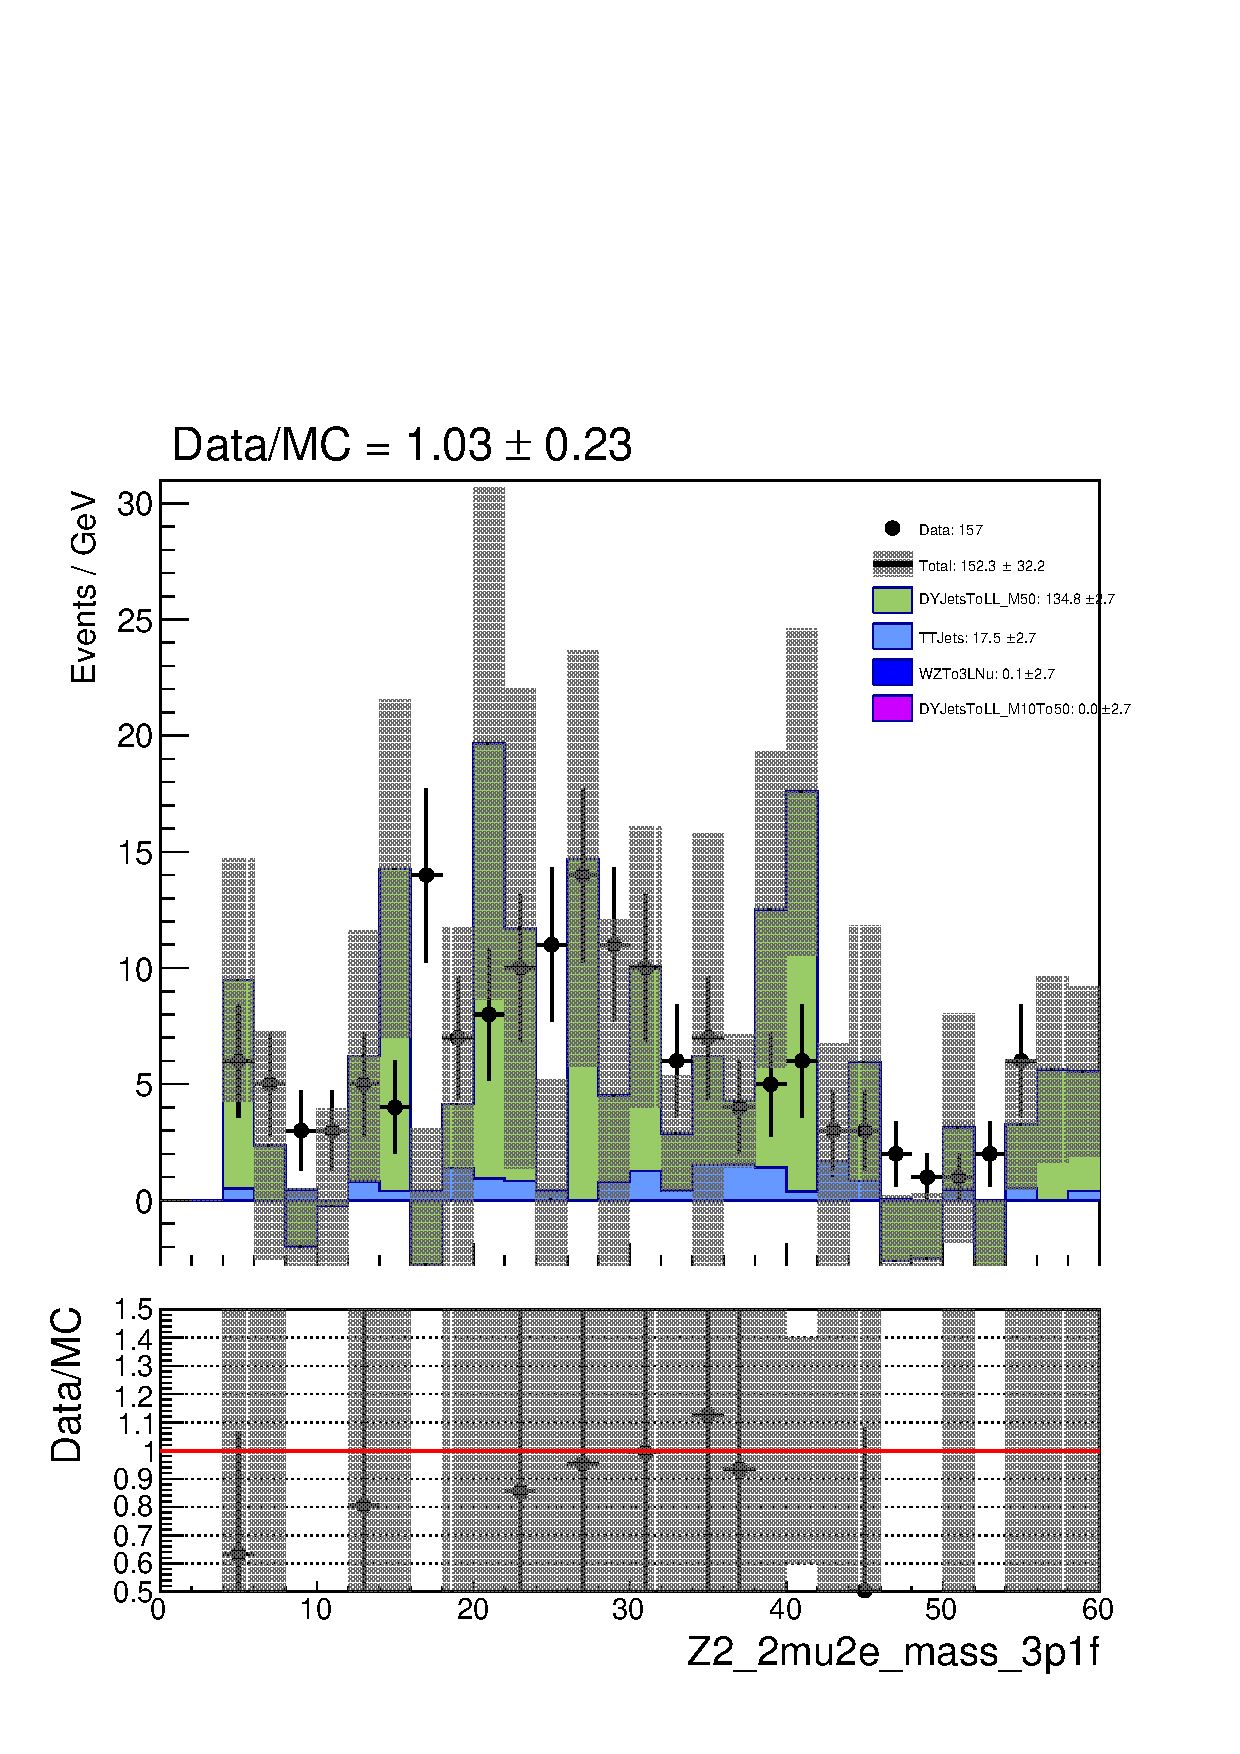
\includegraphics [width=0.45\textwidth] {Figures/RedBkg/3P1F/Z2_2mu2e_mass_3p1f.pdf}}
    {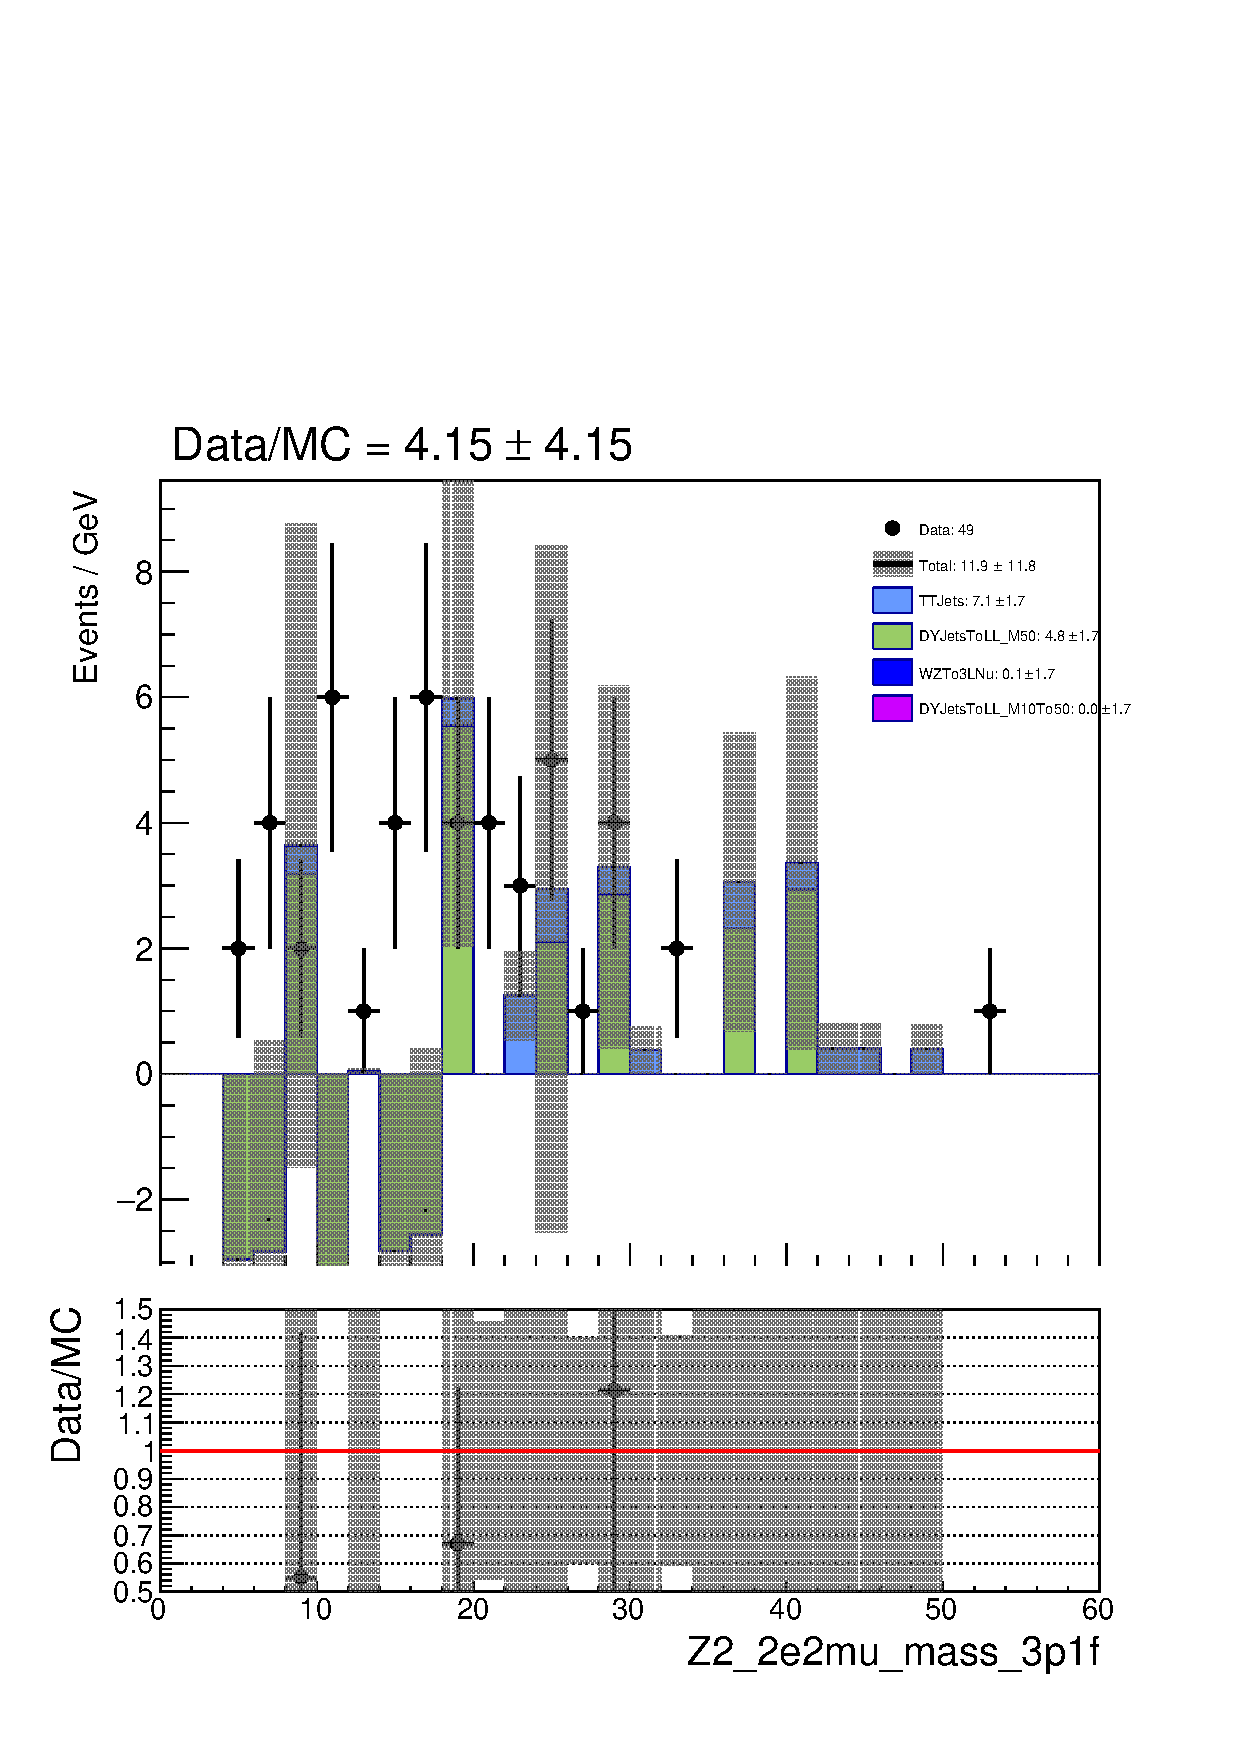
\includegraphics [width=0.45\textwidth] {Figures/RedBkg/3P1F/Z2_2e2mu_mass_3p1f.pdf}} \\
    \caption{
        \mass{Z2} distribution of the events selected in the 3P1F control sample with data in Run 2016, 
        (top left)  $4\mu$ , (top right) $4e$ , (bottom left)  $2\mu2e$ and (bottom right)  $2e2\mu$ channels.
    }
\label{fig:3P1F_dataMC}
\end{center}
\end{figure}

\begin{figure}[!htb]
\begin{center}
    {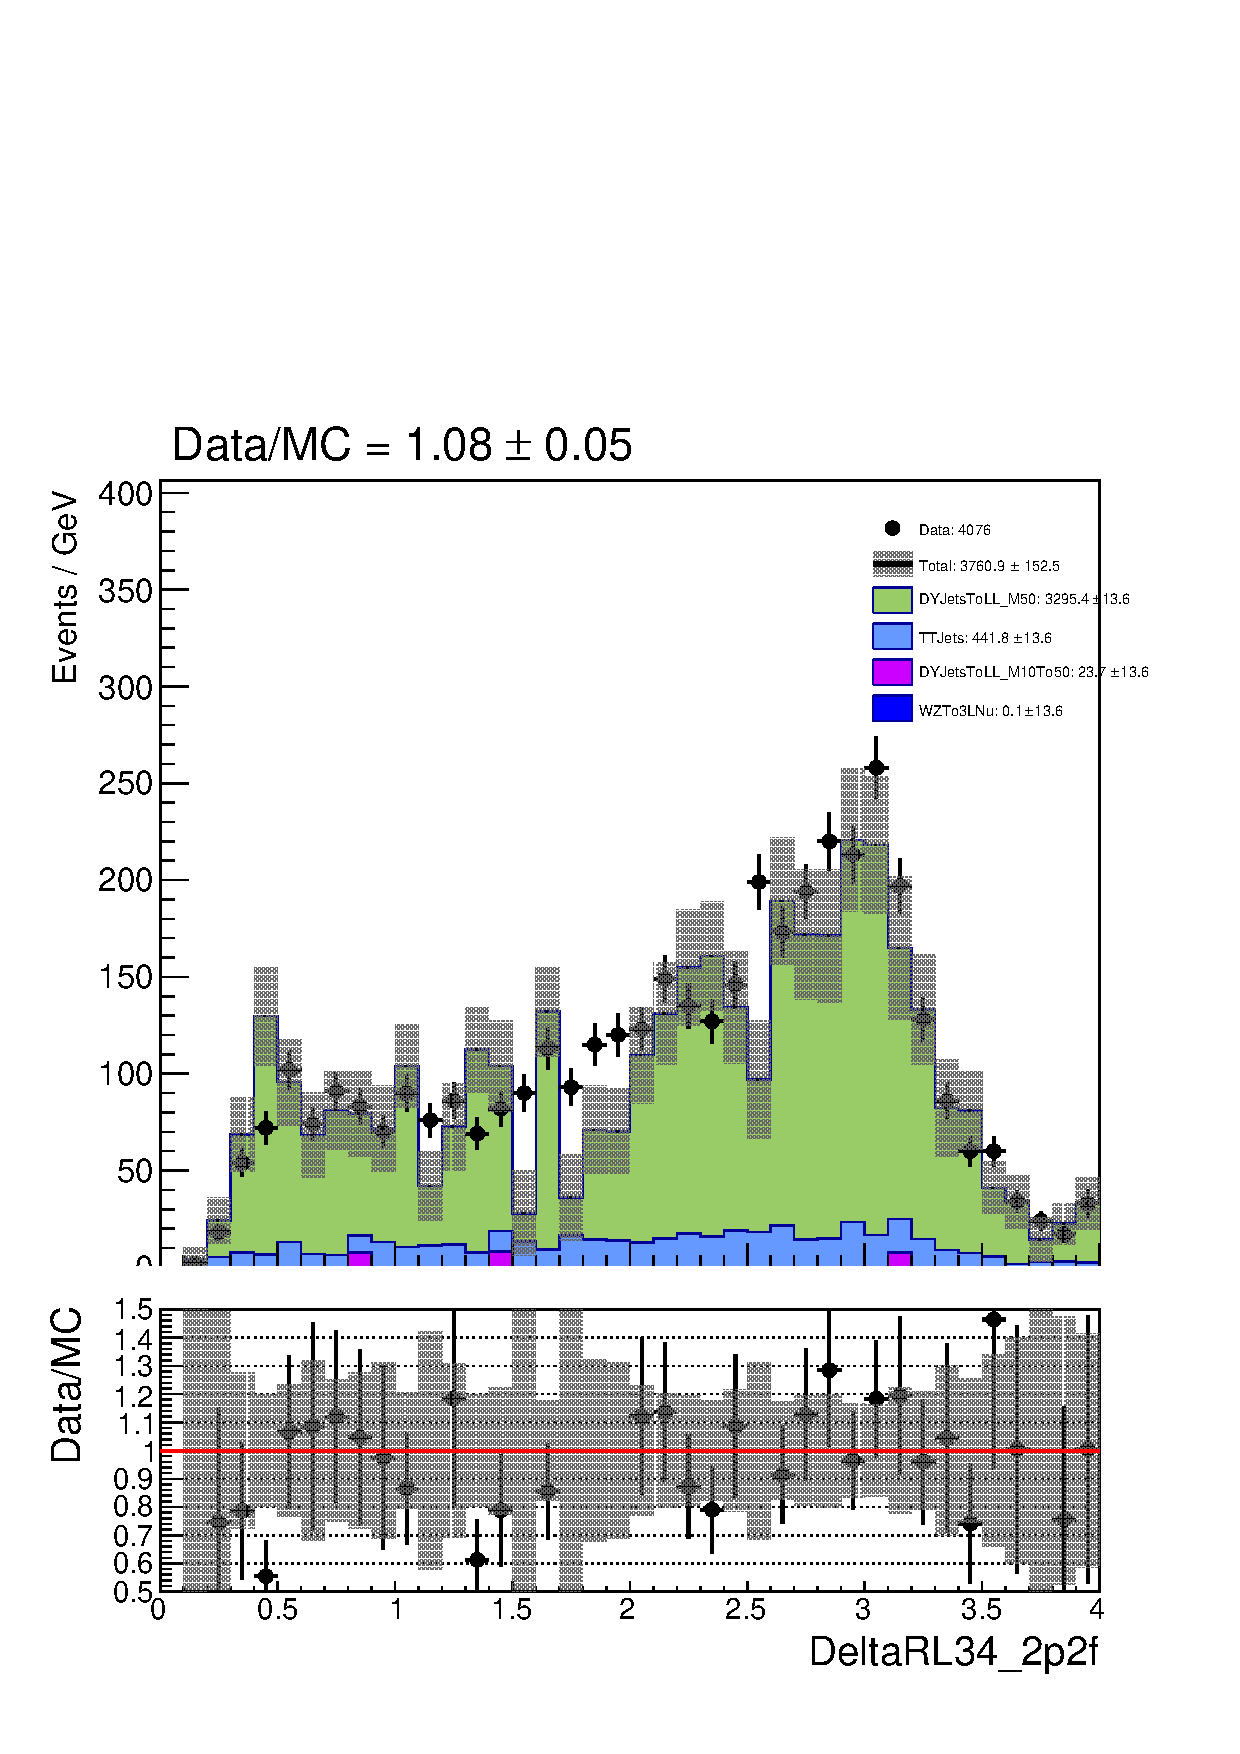
\includegraphics [width=0.45\textwidth] {Figures/RedBkg/2P2F/DeltaRL34_2p2f.pdf}}
    {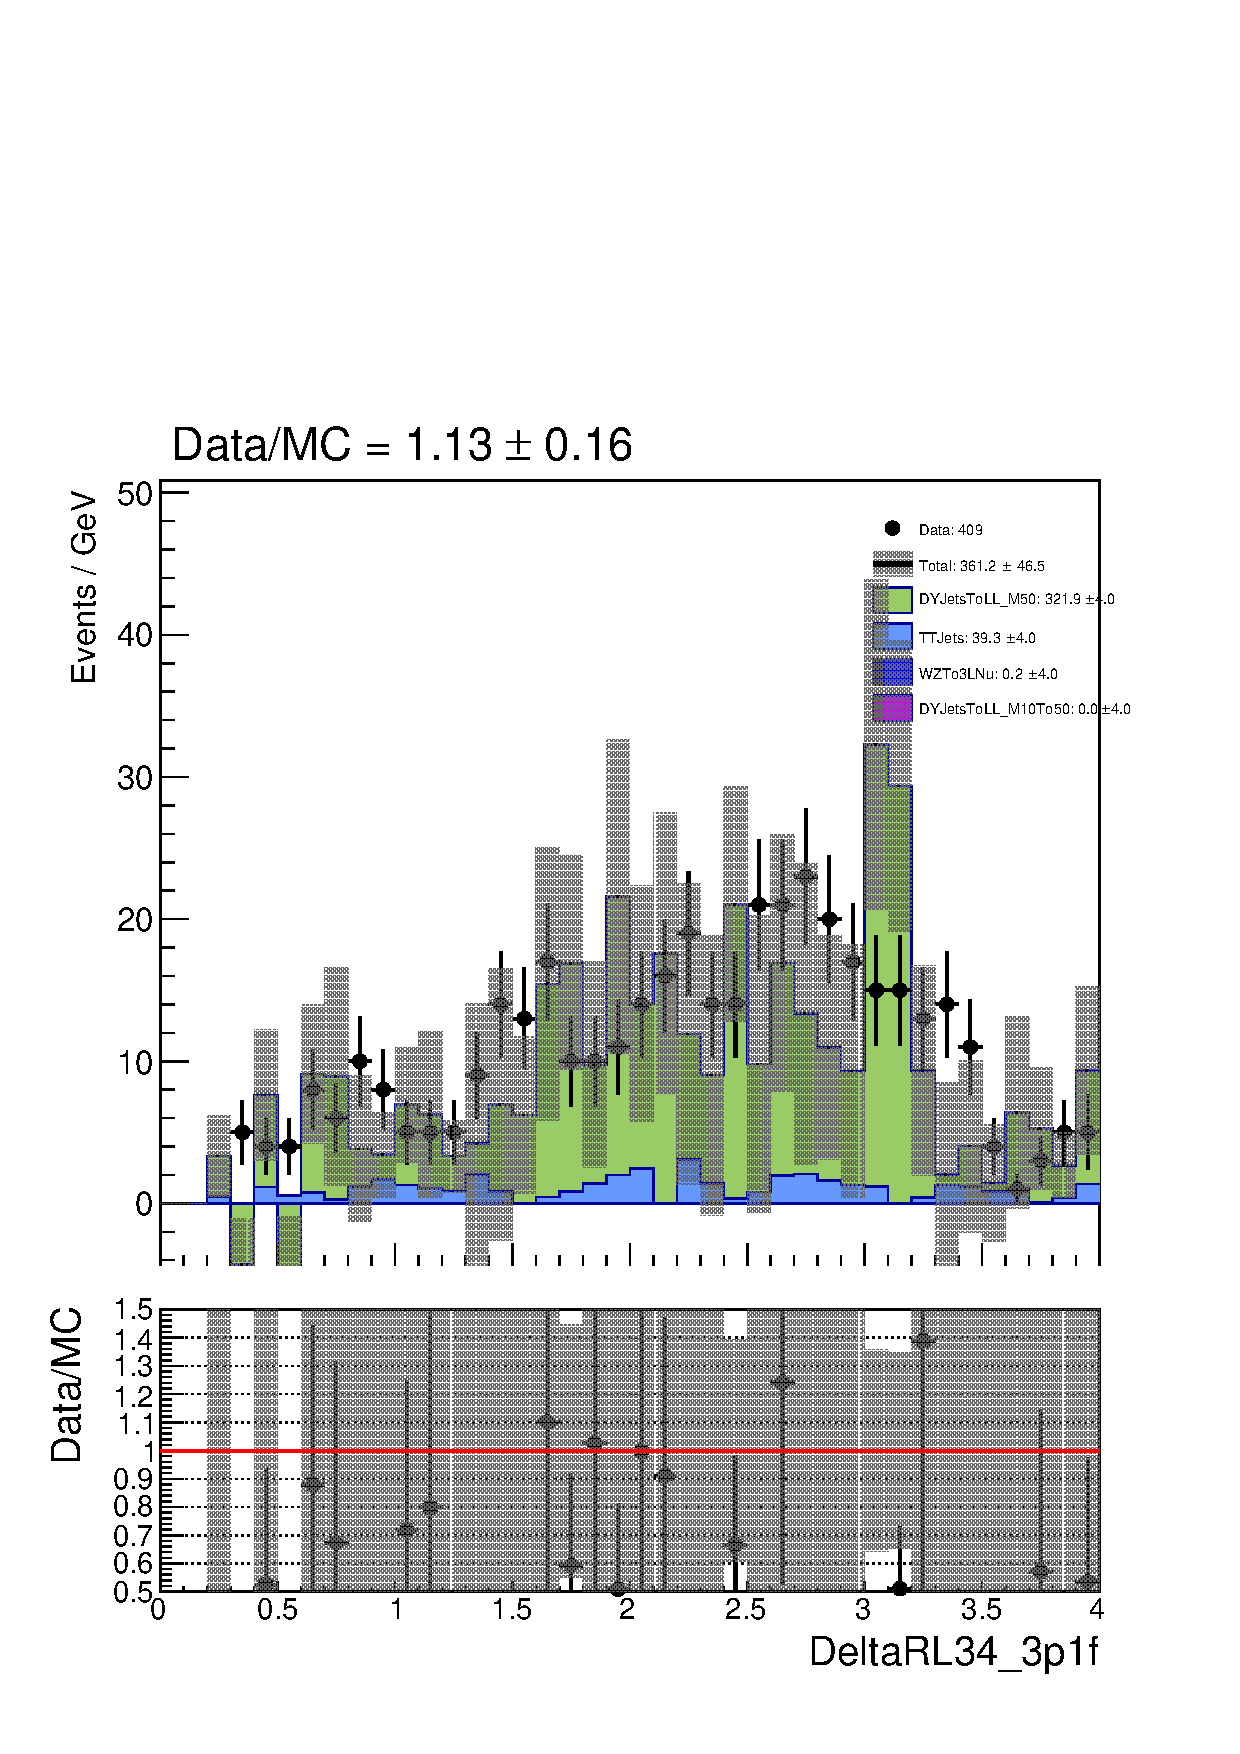
\includegraphics [width=0.45\textwidth] {Figures/RedBkg/3P1F/DeltaRL34_3p1f.pdf}} \\
    \caption{
        Distribution $\Delta R$ of two loose leptons of the events selected in the 2P2F (left) and 3P1F (right) control sample with data in Run 2016. 
    }
\label{fig:DeltaR_dataMC_16}
\end{center}
\end{figure}


\subsubsection{Closure of 3P1F and 2P2F control samples}
Expected numbers of events in the 3P1F control sample can be predicted by the number of events in the 
2P2F control sample, by weighting using fake rates \frEl and \frMu:

\begin{equation} 
\label{eq:Prediction3P1F}
N^{\rm bkg}_{\rm 3P1F} = \sum (\frac{f_{i}}{1-f_{i}}
+ \frac{f_{j}}{1-f_{j}}) N_{\rm 2P2F}
\end{equation} 

Figure~\ref{fig:3P1F_CR} shows the \mass{Z2} distributions in the 3P1F control region and expected predictions from 
the 2P2F control region. Difference between data and predictions from 2P2F are observed, due to photon conversions and 
correlated fake rate of two loose leptons with overlapping isolation cones for low \mass{Z2} in 2P2F. 

\begin{figure}[!htb]
\begin{center}
    {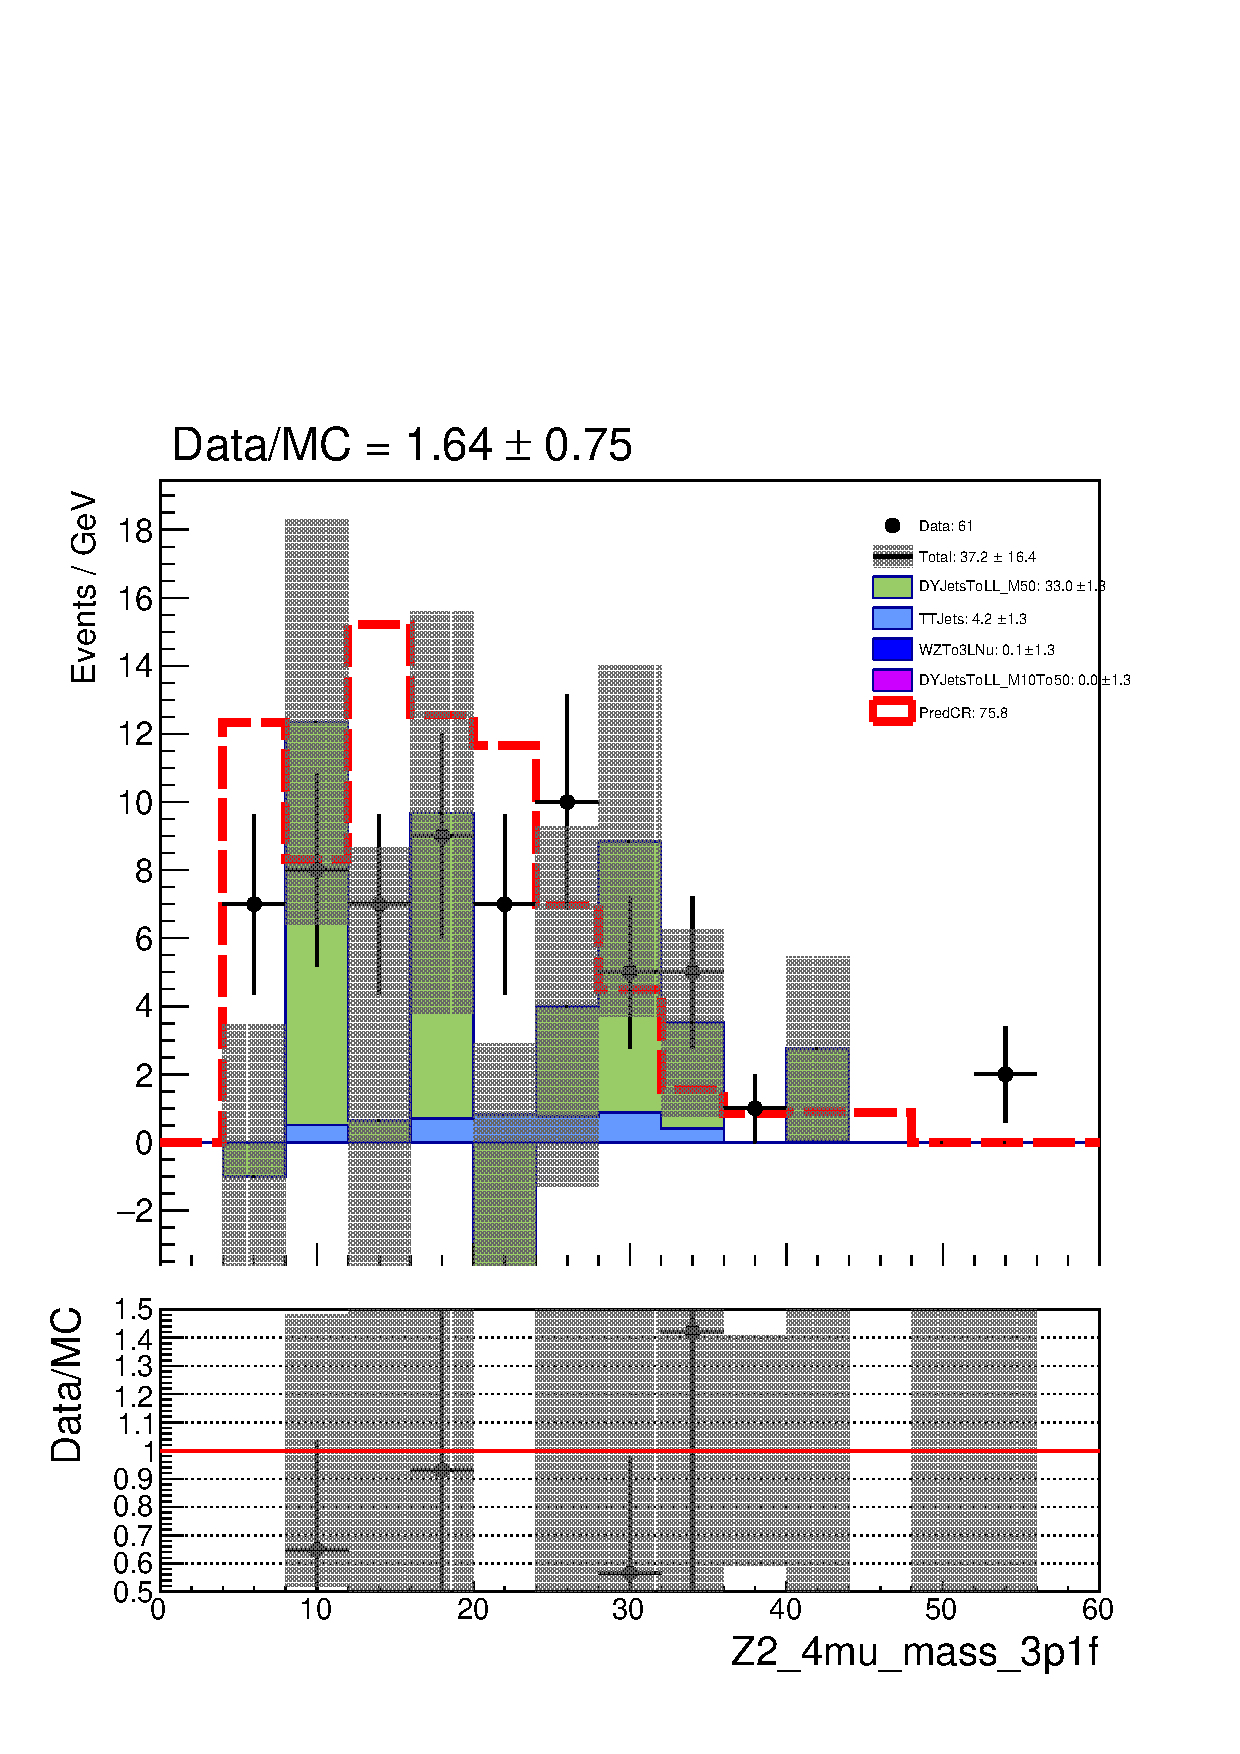
\includegraphics [width=0.45\textwidth] {Figures/RedBkg/3P1F_vs_Pred/Z2_4mu_mass_3p1f.pdf}}
    {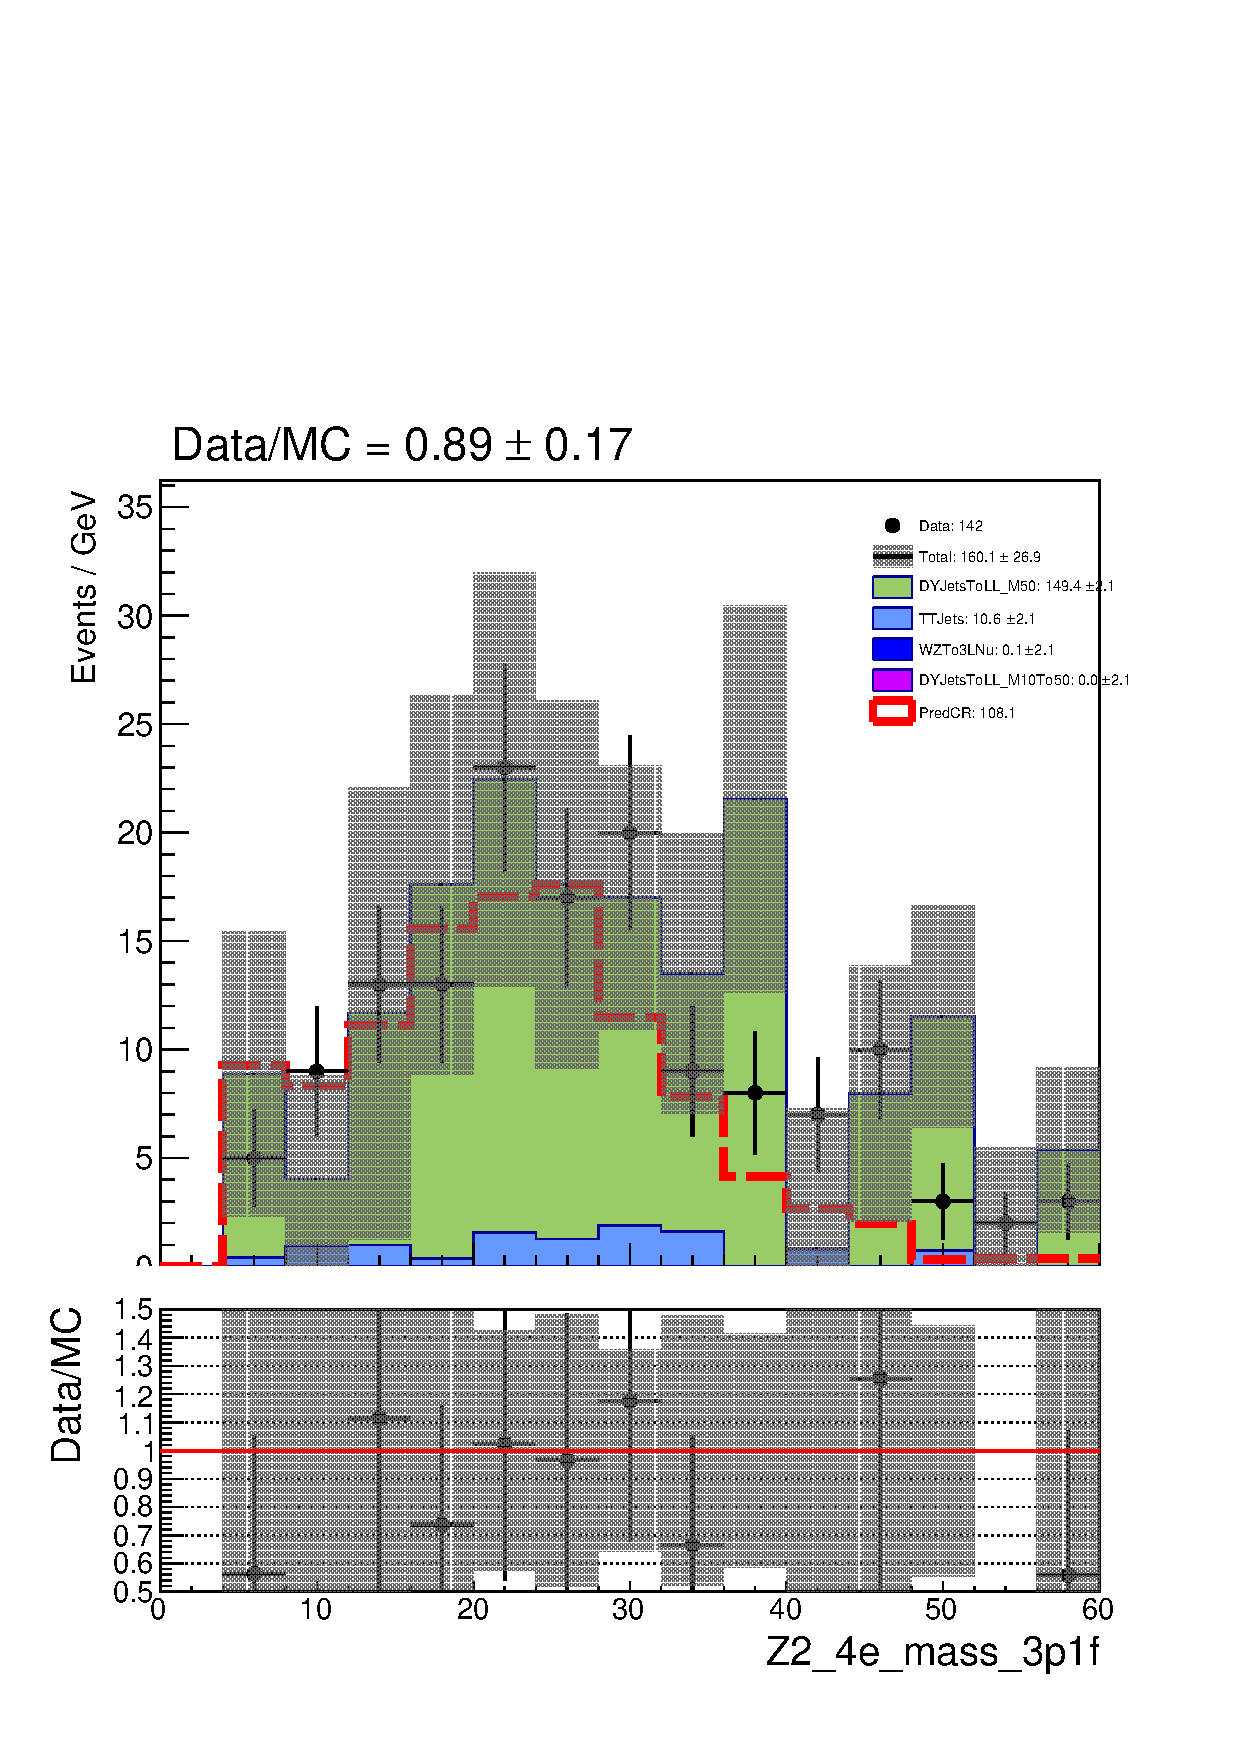
\includegraphics [width=0.45\textwidth] {Figures/RedBkg/3P1F_vs_Pred/Z2_4e_mass_3p1f.pdf}} \\
    {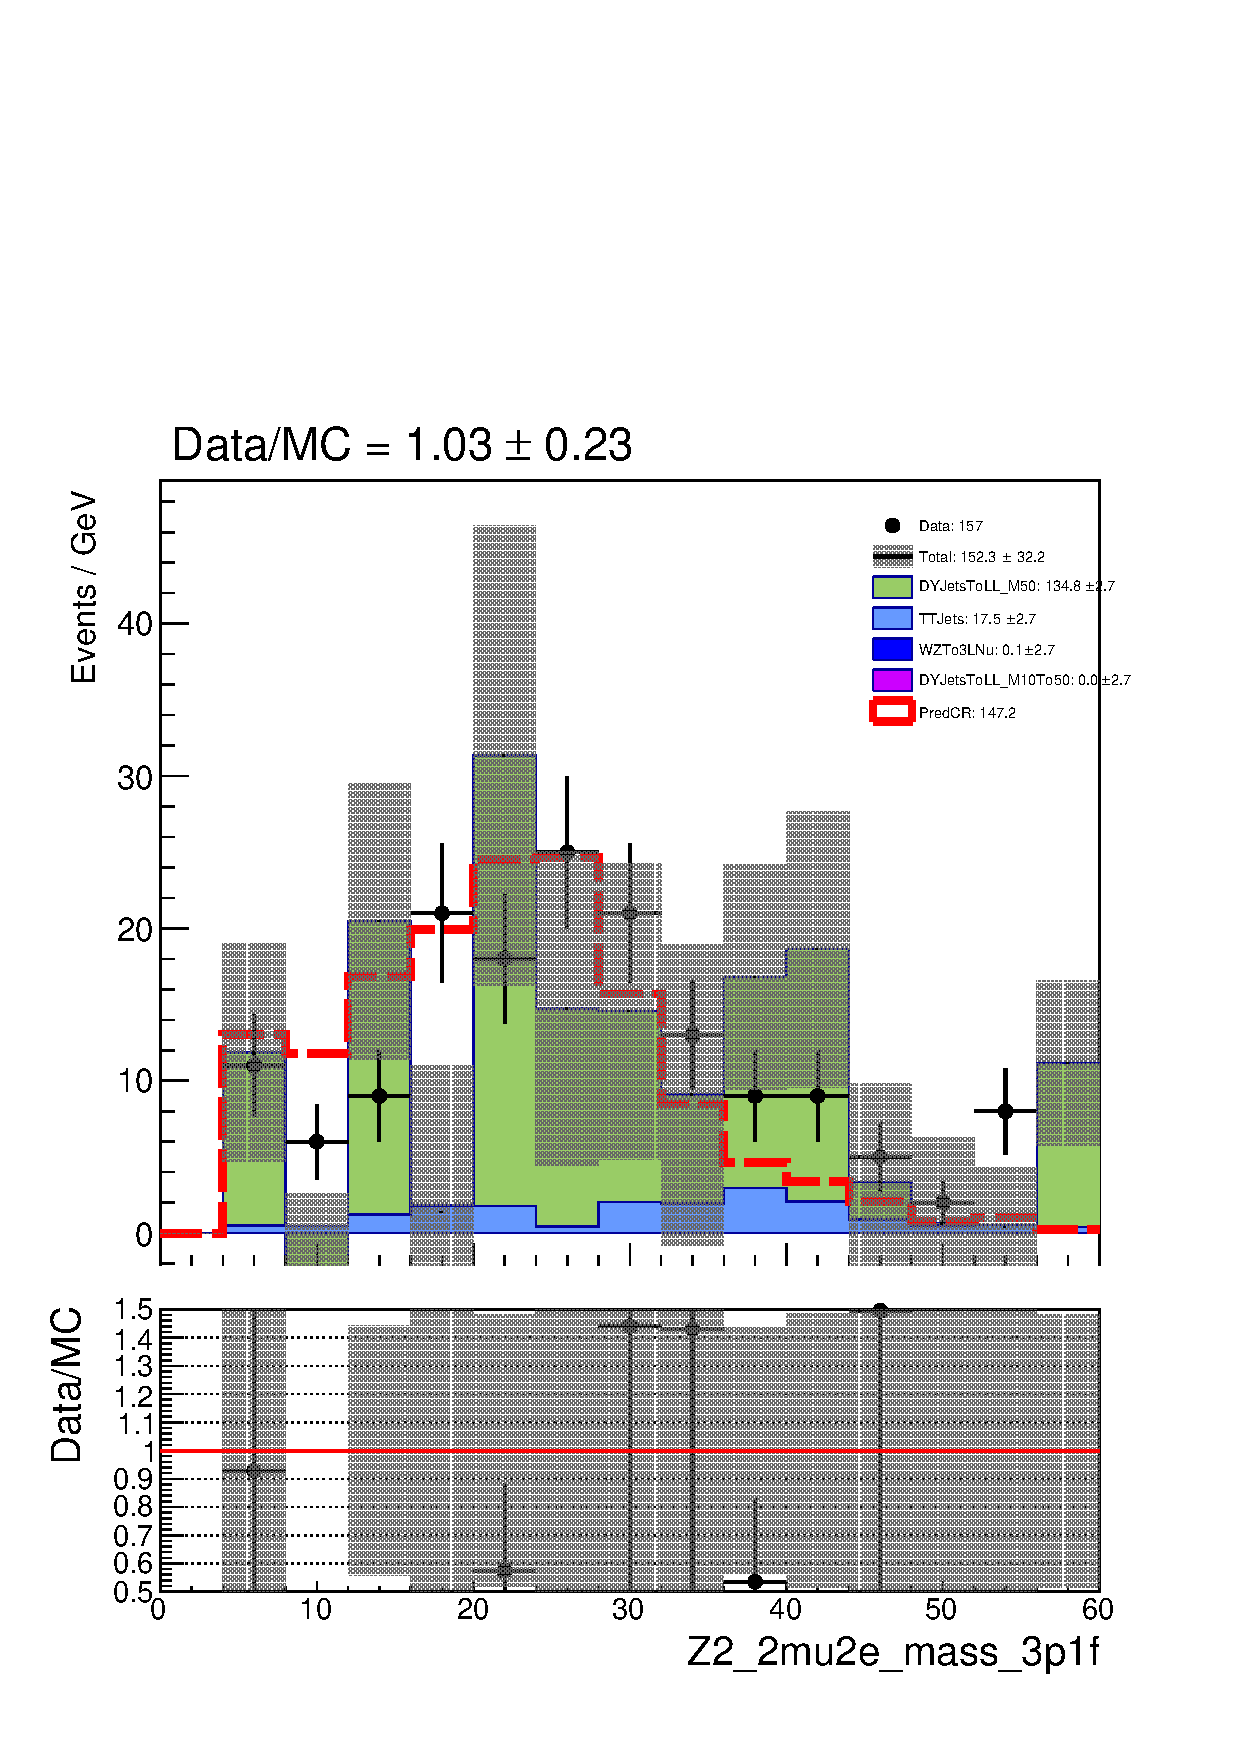
\includegraphics [width=0.45\textwidth] {Figures/RedBkg/3P1F_vs_Pred/Z2_2mu2e_mass_3p1f.pdf}}
    {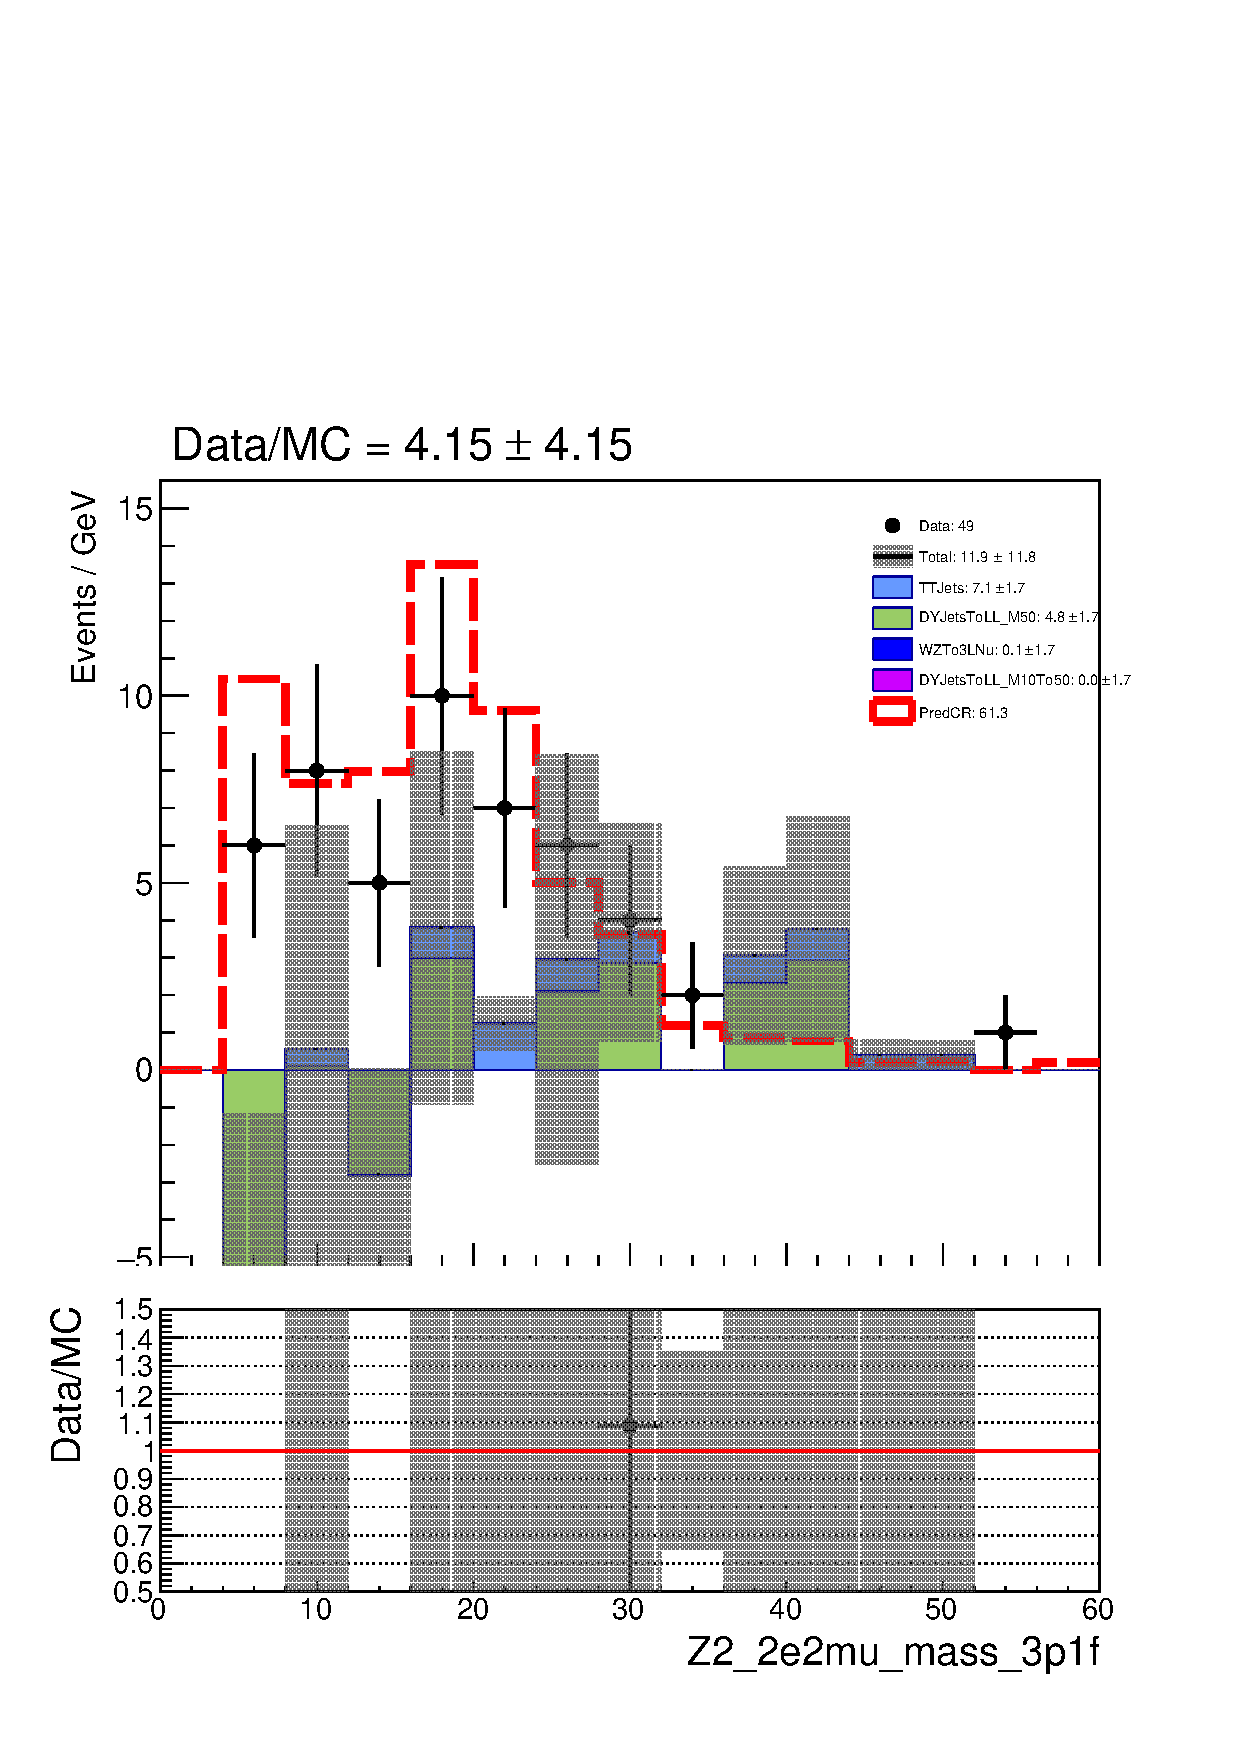
\includegraphics [width=0.45\textwidth] {Figures/RedBkg/3P1F_vs_Pred/Z2_2e2mu_mass_3p1f.pdf}} \\
\caption{
\mass{Z2} distribution of the events selected in the 3P1F control sample in the
$13$~TeV dataset, (top left)  $4\mu$ , (top right) $4e$ , (bottom left)  $2\mu2e$ and (bottom right)  $2e2\mu$ channels.
}
\label{fig:3P1F_CR}
\end{center}
\end{figure}

\subsubsection{Prediction for signal region}
To correct for potential bias of photon conversions, both 3P1F and 2P2F control samples are used to extract the \zx prediction 
in the signal region. Mathematically, the prediction can be written by a sum of two terms:
\begin{itemize}
\item a ``2P2F component", obtained from the number of
  events observed in the 2P+2F control region, $N_{\rm 2P2F}$, by
  weighting each event in that region with the factor
  $\frac{f_{i}}{1-f_{i}} \frac{f_{j}}{1-f_{j}}$, where $f_{i}$ and
  $f_{j}$ correspond to the fake ratios of the two loose leptons.
\item a ``3P1F component", obtained from the
   difference between the number of observed events in the 3P+1F control
   region, $N_{\rm 3P1F}$, and the expected contribution from the 2P+2F
   region and ZZ processes in the signal region, $N^{\rm ZZ}_{\rm 3P1F} +
   N^{\rm bkg}_{\rm 3P1F}$. The $N^{\rm bkg}_{\rm 3P1F}$ is given by 
   equation \ref{eq:Prediction3P1F} and $N^{\rm ZZ}_{\rm 3P1F}$ is the
   contribution from $ZZ$ which is taken from the simulation. 
   The difference $N_{\rm 3P1F} -  N^{\rm bkg}_{\rm 3P1F} - N^{\rm ZZ}_{\rm 3P1F}$,
   which may be negative,
   is obtained for each $(p_T, \eta)$ bin of the ``F" lepton, and is weighted 
   by $\frac{f_i} {1 - f_i}$, where $f_i$ denotes the fake rate of
   this lepton.
   This ``3P1F component" accounts for the contribution of reducible background
   processes with only one fake lepton (like \wz events), and for the contribution
   of other processes (e.g. photon conversions) that are not properly estimated
   by the 2P2F component, because of the fake rates used.
\end{itemize}
Hence, the formula can be written as:
\begin{equation} 
\label{eq:PredictionSR}
N^{bkg}_{\rm SR} = \sum \frac{f_{i}}{(1-f_{i})} (N_{\rm 3P1F} - N^{\rm
bkg}_{\rm 3P1F} - N^{\rm ZZ}_{\rm 3P1F})
+ \sum \frac{f_{i}}{(1-f_{i})} \frac{f_{j}}{(1-f_{j})}N_{\rm 2P2F} \end{equation}
and it is equivalent to
\begin{equation}
\label{eq:PredictionSR2}
N^{bkg}_{\rm SR}= (1-\frac{N_{3P1F}^{ZZ}}{N_{3P1F}})\sum_j^{N_{3P1F}}\frac{f_a^j}{1-f_a^j} - \sum_i^{N_{2P2F}}\frac{f_3^i}{1-f_3^i}\frac{f_4^i}{1-f_4^i}
\end{equation}

\subsubsection{Validation with the \mass{4\ell} sideband}
Dedicated validation with two sidebands are performed to demonstrate robustness of the method against correlated fake 
rates at low \massZ2 regions.

Two \mass{4\ell} sidebands ($105~\GeV < \mass{4l} < 118~\GeV$ and $130~\GeV < \mass{4l} < 140~\GeV$) are defined adjacent 
to the signal region to check the \zx background against data. The \mass{4\ell} sidebands are selected with the same selection 
as the signal region, except the changes in the \mass{4\ell} cut. Figure~\ref{fig:m4l_SB} shows the data/MC distributions in 
\mass{Z2} for these two sidebands. It is observed that for $\mass{Z2} < 12~\GeV$, the \zx background has a small contribution 
to the total background and reasonable data and MC agreements are observed.

\begin{figure}[!htb]
\begin{center}
    {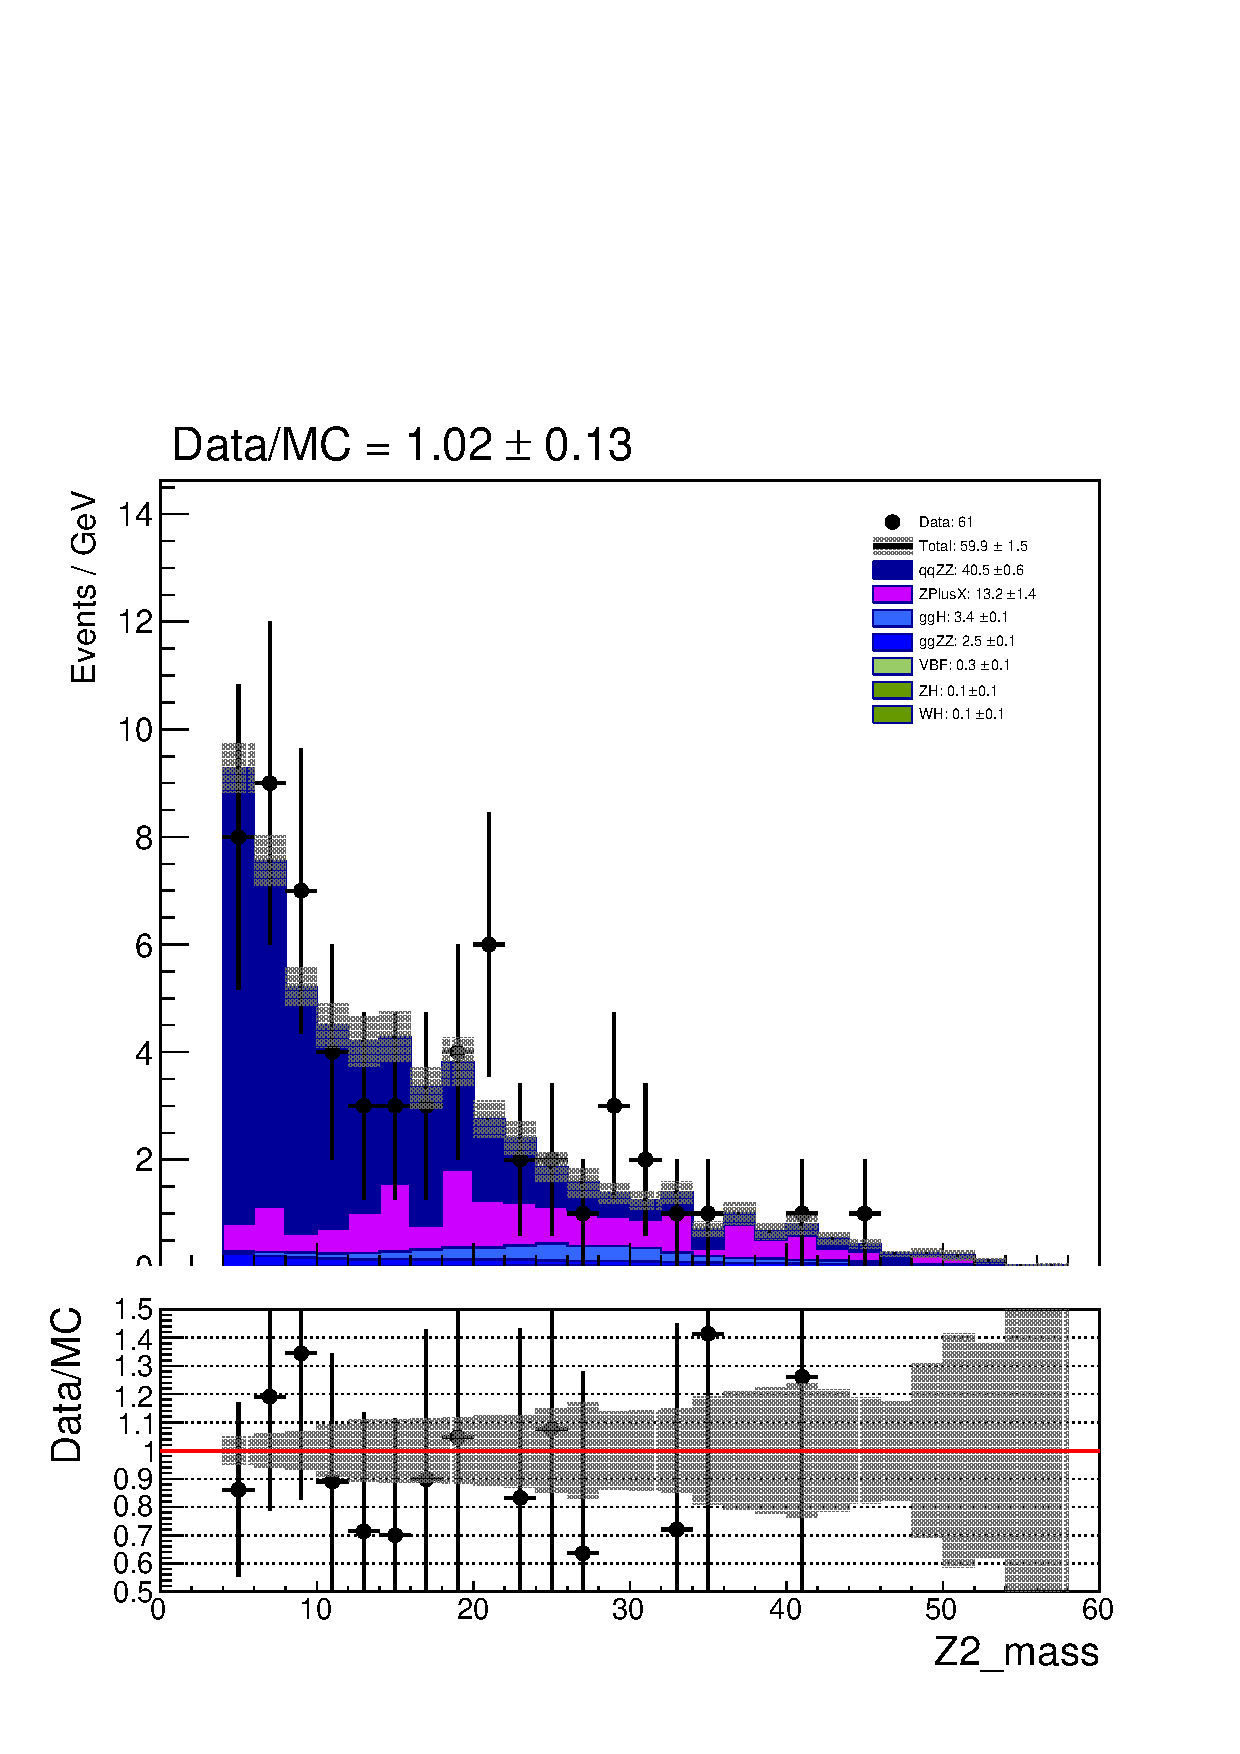
\includegraphics [width=0.45\textwidth] {Figures/RedBkg/m4lSB/Z2_mass_m4l105To118}}
    {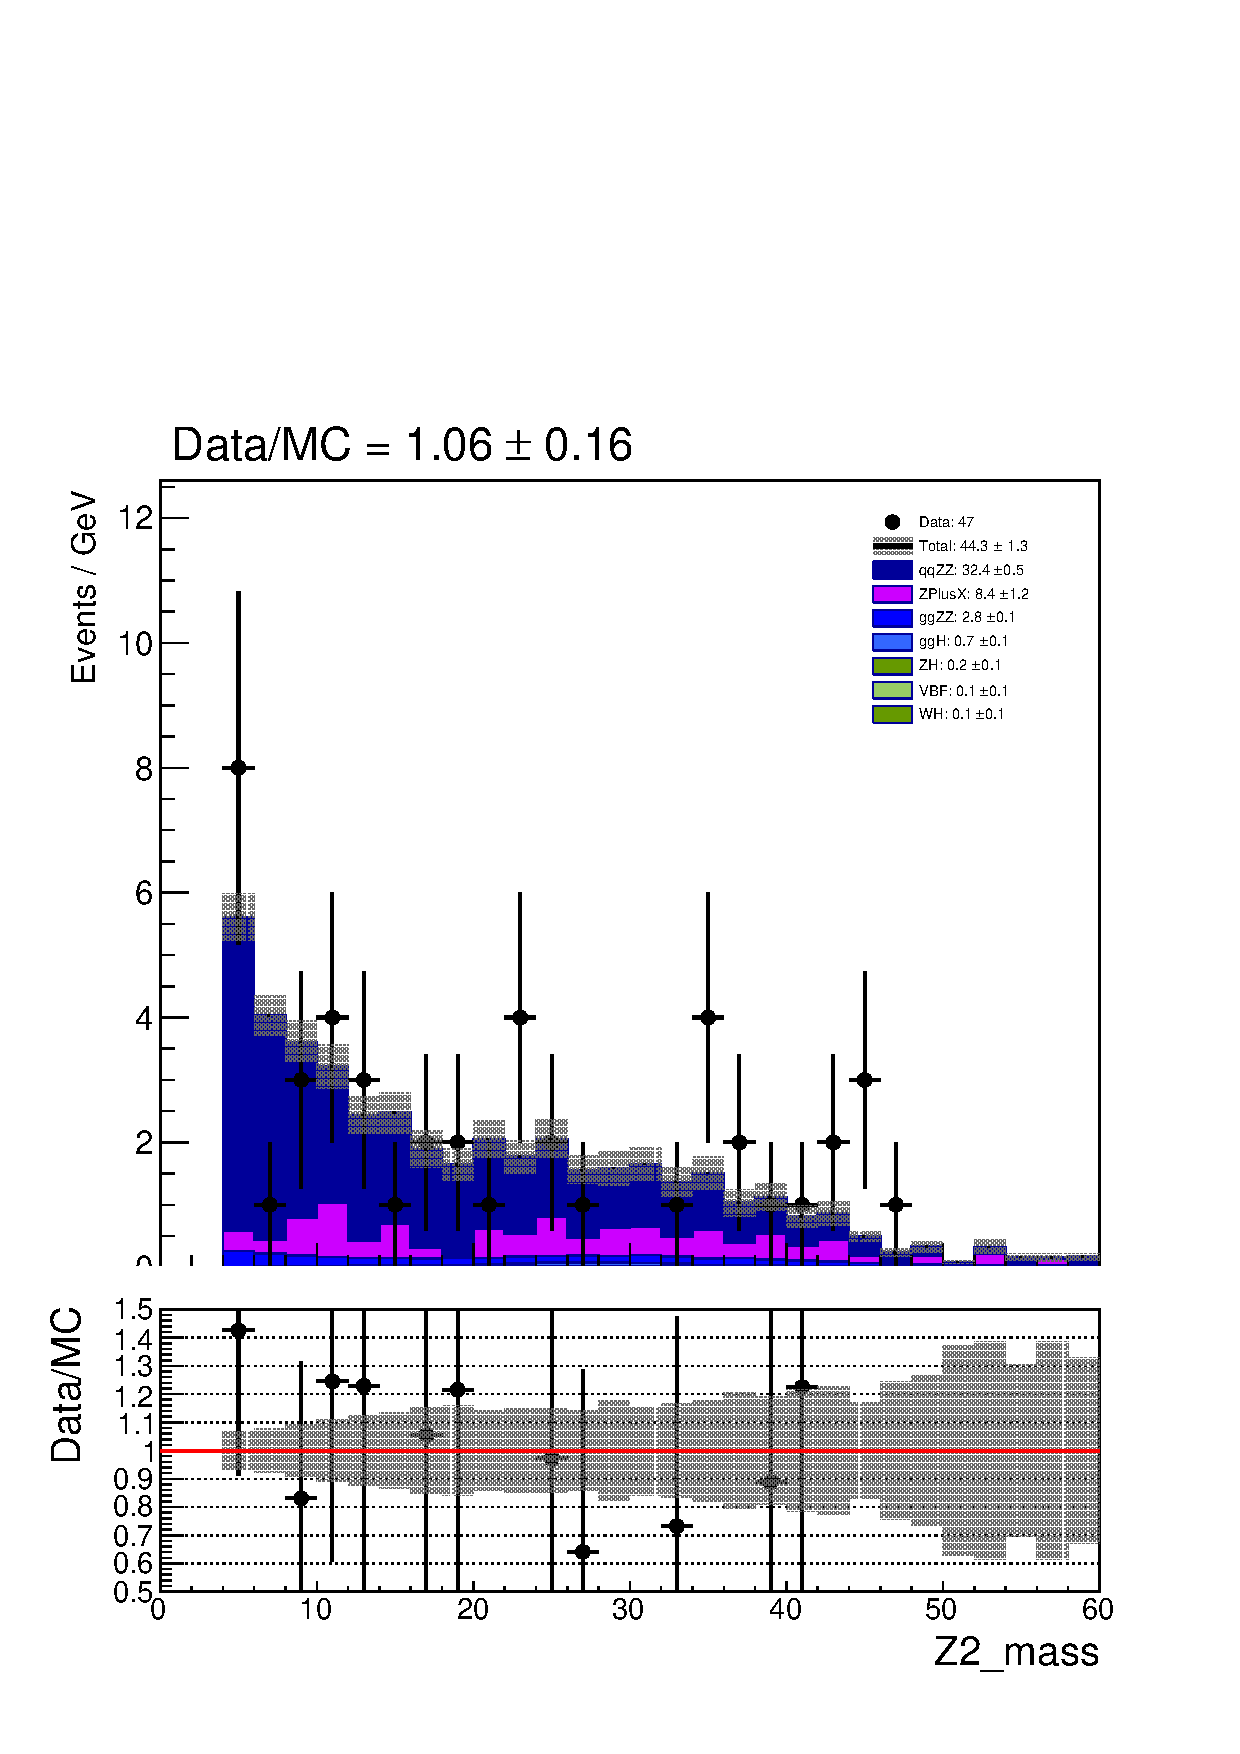
\includegraphics [width=0.45\textwidth] {Figures/RedBkg/m4lSB/Z2_mass_m4l130To140}} \\
\caption{
    \mass{Z2} distribution of the events selected in the \mass{4\ell} control sample in the
    $13~\TeV$ dataset, (left)  $105~\GeV < \mass{4l} < 118~\GeV$ , (right) $130~\GeV < \mass{4l} < 140~\GeV$.
}
\label{fig:m4l_SB}
\end{center}
\end{figure}

\subsubsection{Validation with the Wrong-Flavour-Charge (WFC) sideband}
Besides the \mass{4\ell} sidebands, the WFC control region is also defined to check the closure 
between data and prediction with the OS method. The WFC control region is selected with the same selections as the signal 
region, except that the Z1 and Z2 candidates are formed by pairs of leptons either with same charges or different flavours.
Three control regions are defined subsequently: 4P0F, 3P1F, 2P2F control regions, depending on whether each lepton forming 
the Z2 candidate satisfies the tight selection criteria.
Similar to the nominal analysis, both the 3P1F and 2P2F control samples are used to predict \zx background contributions in 
the 4P0F control region. In addition to the non-prompt \zx background, physics processes with four prompt leptons, such as 
\qqZZ can contributes to this control region.
Figure~\ref{fig:WFC} shows a comparison of data and prediction of this control sample. Data agree with the predictions
within $20\%$.

\begin{figure}[!htb]
\begin{center}
    {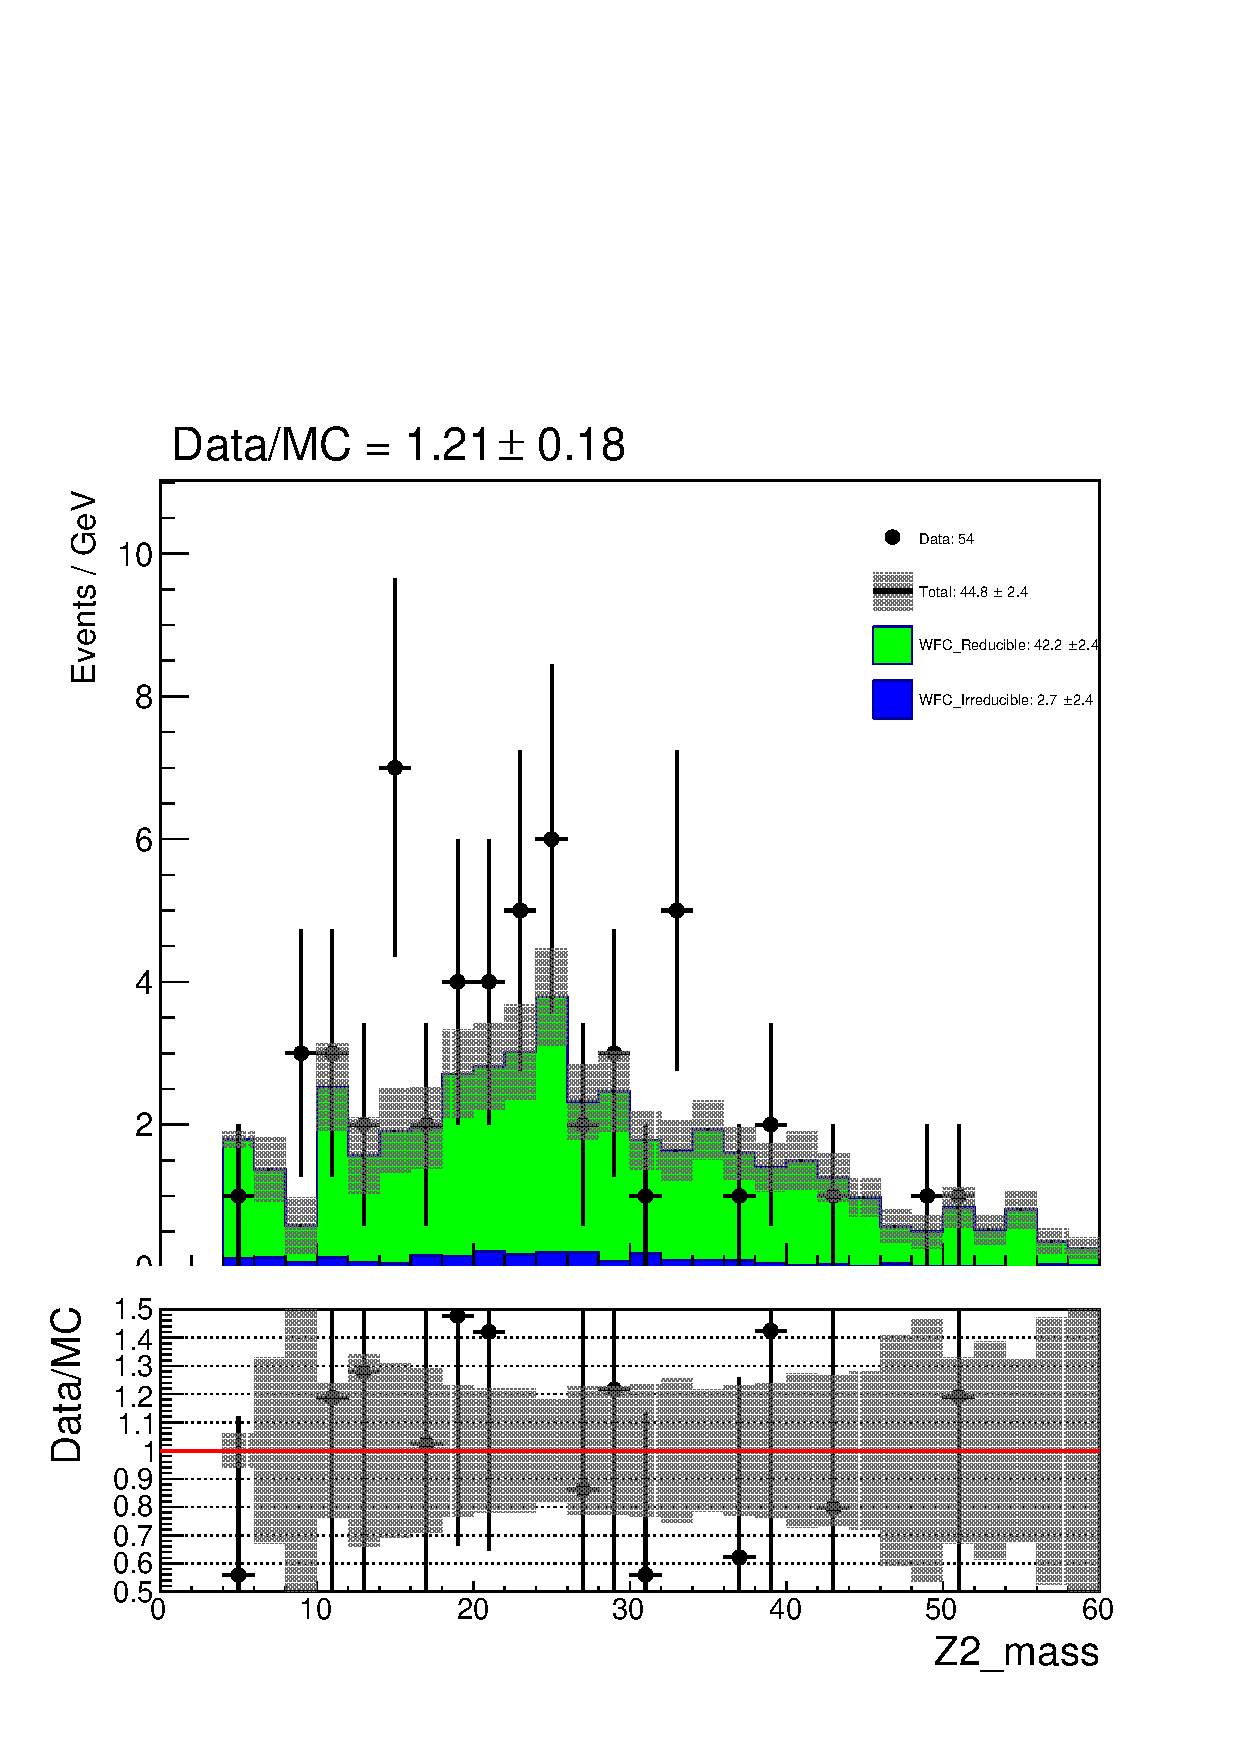
\includegraphics [width=0.8\textwidth] {Figures/RedBkg/WFC/Z2_mass}}
\caption{
    \mass{Z2} distribution of the events selected in the WFC control sample in the$13~\TeV$ dataset.
}
\label{fig:WFC}
\end{center}
\end{figure}

\subsubsection{Systematic uncertainty}
One source of systematic uncertainties of the OS method could potentially arise from different compositions of 
background processes between the fake rate measurement and application regions. This uncertainty is estimated 
by measuring, in simulation, fake rates of each background process in the measurement region. Predictions 
obtained with different fake rates derived from simulation are compared to predictions obtained by the nominal 
fake rates. Differences observed are used as a measure of the systematic uncertainty. Effects of this systematic 
uncertainty are typically about XX\% for $4e$, XX\% for $2e2\mu$ and XX\% for $4\mu$ final state.

Another source of systematic uncertainty comes from the assumption of factorized fake rates for two loose leptons 
in the 2P2F control region. To estimate this effect, two extreme scenarios are considered for events with 
$\Delta R_{Z2} < 0.6$:
\begin{enumerate}
    \item Isolation activities are uniform in each isolation cone of the two loose leptons. \label{list:fr_uniform} 
    \item Isolation activities are contained only in only one of the two isolation cones of the two loose leptons. \label{list:fr_one} 
\end{enumerate}
For Case~\ref{list:fr_uniform}, the sum and products of the fake rates can be corrected as:
\begin{equation}
\label{eq:syst_corrfr_sum}
\left(1-f_A\right)\left(1-f_B\right) \rightarrow \left(1-f_A\right)\left(1-f_B\right) \left(\frac{\Delta R_{AB}}{2R_{iso}} \right)^2 + \sqrt{\left(1-f_A\right)\left(1-f_B\right)} \left(1-\frac{\Delta R_{AB}}{2R_{iso}} \right)
\end{equation}

\begin{equation}
\label{eq:syst_corrfr_prod}
f_A f_B \rightarrow f_A f_B \left(\frac{\Delta R_{AB}}{2R_{iso}} + \sqrt{f_A f_B} (1-\frac{\Delta R_{AB}}{2R_{iso}}) \right)
\end{equation}
where $\Delta R_{AB}$ is $\Delta R$ between lepton A and B, and $\Delta R_{iso}$ is the isolation cone used.
For Case~\ref{list:fr_one}, the event is assumed to be from the 3P1F control region and the fake rate corresponding to the 
loose lepton with larger isolation value is used to reweight this event. Effects of correlated fake rates are then 
estimated by the differences on the prediction in the signal region by assuming Case~\ref{list:fr_uniform} and 
Case~\ref{list:fr_one}, and are typically about XX\% for $4e$, XX\% for $2e2\mu$ and XX\% for $4\mu$ final state.
